%%%%%%%%%%%%%%%%%%%%%%%%%%%%%%%%%%%%%%%%%%%%%%%%%%%%%%%%%%%%%%%%%%%%%%%%%
%  Zawartość: Główny plik szablonu pracy dyplomowej (magisterskiej/inżynierskiej).
%  Opracował: Tomasz Kubik <tomasz.kubik@pwr.edu.pl>
%  Data: kwiecień 2016
%  Wersja: 0.2
%%%%%%%%%%%%%%%%%%%%%%%%%%%%%%%%%%%%%%%%%%%%%%%%%%%%%%%%%%%%%%%%%%%%%%%%%

\documentclass[a4paper,onecolumn,oneside,12pt,extrafontsizes]{memoir}
% W celu przygotowania wydruku do archiwum należy przesłonić komendę powyższą
% dwoma poniższymi komendami:
% \documentclass[a4paper,onecolumn,twoside,10pt]{memoir} 
% \renewcommand{\normalsize}{\fontsize{8pt}{10pt}\selectfont}

%\usepackage[cp1250]{inputenc} % jeśli kodowanie edytowanych plików to cp1250 
\usepackage[utf8]{inputenc} % jeśli kodowanie edytowanych plików to UTF8
\usepackage[T1]{fontenc}
\usepackage[polish]{babel}
%\DisemulatePackage{setspace}
\usepackage{setspace}
\usepackage{subfig}
\usepackage{tabularx}
\usepackage{color,calc}
%\usepackage{soul} % pakiet z komendami do podkreślania tekstu

%moje
\usepackage{algorithm}
\usepackage{dirtree}
\usepackage{amsmath}
\usepackage[noend]{algpseudocode}

\usepackage{ebgaramond} % pakiet z czcionkami garamond, potrzebny tylko do strony tytułowej, musi wystąpić przed pakietem tgtermes

%% Aby uzyskać polskie literki w pdfie (a nie zlepki) korzystamy z pakietu czcionek tgterms. 
%% W pakiecie tym są zdefiniowane klony czcionek Times o kształtach: normalny, pogrubiony, italic, italic pogrubiony.
%% W pakiecie tym brakuje czcionki o kształcie: slanted (podobny do italic). 
%% Jeśli w dokumencie gdzieś zostanie zastosowana czcionka slanted (np. po użyciu komendy \textsl{}), to
%% latex dokona podstawienia na czcionkę standardową i zgłosi to w ostrzeżeniu (warningu).
%% Ponadto tgtermes to czcionka do tekstu. Wszelkie matematyczne wzory będą sformatowane domyślną czcionką do wzorów.
%% Jeśli wzory mają być sformatowane z wykorzystaniem innych czcionek, trzeba to jawnie zadeklarować.

%% Po zainstalowaniu pakietu tgtermes może będzie trzeba zauktualizować informacje 
%% o dostępnych fontach oraz mapy. Można to zrobić z konsoli (jako administrator)
%% initexmf --admin --update-fndb
%% initexmf --admin --mkmaps

\usepackage{tgtermes}   
\renewcommand*\ttdefault{txtt}

% We wcześniejszej wersji szablonu korzystano z innych czcionek. Dla celów historycznych pozostawiono je w komentarzu
%\usepackage{mathptmx} % pakiet będący następcą pakietów times and mathptm, niestety polskie literki są zlepkami
%\usepackage{newtxtext,newtxmath} % pakiety dostarczające Times dla tekstów i wzorów matematycznych,  
%                                  rozwiązuje problemy występujące w mathptmx, ale wymaga zainstalowania
%                                  dodatkowych pakietów oraz uruchomienia updmap (konsola administratora)
%                                  niestety polskie literki są zlepkami
%\usepackage{newtxmath,tgtermes} % można też połączyć czcionki do tekstu i czcionki do wzorów

\usepackage{listings} % pakiet do prezentacji kodu. 
%Wcześniej był problem z polskimi znakami w otoczeniu lstlisting, stąd pozostawiono w komentarzu zastosowane wtedy rozwiązanie: 
\lstset{literate=%-
{ą}{{\k{a}}}1 {ć}{{\'c}}1 {ę}{{\k{e}}}1 {ł}{{\l{}}}1 {ń}{{\'n}}1 {ó}{{\'o}}1 {ś}{{\'s}}1 {ż}{{\.z}}1 {ź}{{\'z}}1 {Ą}{{\k{A}}}1 {Ć}{{\'C}}1 {Ę}{{\k{E}}}1 {Ł}{{\L{}}}1 {Ń}{{\'N}}1 {Ó}{{\'O}}1 {Ś}{{\'S}}1 {Ż}{{\.Z}}1 {Ź}{{\'Z}}1 }%{\ \ }{{\ }}1}

% Choć możliwe jest zastosowanie różnych pakietów formatujących tabele, zaleca się tego nie robić.
%\usepackage{longtable}
%\usepackage{ltxtable}
%\usepackage{tabulary}

%%%%%%%%%%%%%%%%%%%%%%%%%%%%%%%%%%%%%%%%%%%%%%%%%%%
%% Ustawienia odpowiedzialne za sposób łamania dokumentu
%% i ułożenie elementów pływających
%%%%%%%%%%%%%%%%%%%%%%%%%%%%%%%%%%%%%%%%%%%%%%%%%%%
%\hyphenpenalty=10000		% nie dziel wyrazów zbyt często
\clubpenalty=10000      %kara za sierotki
\widowpenalty=10000  % nie pozostawiaj wdów
\brokenpenalty=10000		% nie dziel wyrazów między stronami
\exhyphenpenalty=999999		% nie dziel słów z myślnikiem
\righthyphenmin=3			% dziel minimum 3 litery

%\tolerance=4500
%\pretolerance=250
%\hfuzz=1.5pt
%\hbadness=1450

\renewcommand{\topfraction}{0.95}
\renewcommand{\bottomfraction}{0.95}
\renewcommand{\textfraction}{0.05}
\renewcommand{\floatpagefraction}{0.35}

%%%%%%%%%%%%%%%%%%%%%%%%%%%%%%%%%%%%%%%%%%%%%%%%%%%
%%  Ustawienia rozmiarów: tekstu, nagłówka i stopki, marginesów
%%  dla dokumentów klasy memoir 
%%%%%%%%%%%%%%%%%%%%%%%%%%%%%%%%%%%%%%%%%%%%%%%%%%%
\setlength{\headsep}{10pt} 
\setlength{\headheight}{13.6pt} % wartość baselineskip dla czcionki 11pt tj. \small wynosi 13.6pt
\setlength{\footskip}{\headsep+\headheight}
\setlength{\uppermargin}{\headheight+\headsep+1cm}
\setlength{\textheight}{\paperheight-\uppermargin-\footskip-1.5cm}
\setlength{\textwidth}{\paperwidth-5cm}
\setlength{\spinemargin}{2.5cm}
\setlength{\foremargin}{2.5cm}
\setlength{\marginparsep}{2mm}
\setlength{\marginparwidth}{2.3mm}
%\settrimmedsize{297mm}{210mm}{*}
%\settrims{0mm}{0mm}	
\checkandfixthelayout[fixed] % konieczne, aby się dobrze wszystko poustawiało
%%%%%%%%%%%%%%%%%%%%%%%%%%%%%%%%%%%%%%%%%%%%%%%%
%%  Ustawienia odległości linii, wcięć, odstępów
%%%%%%%%%%%%%%%%%%%%%%%%%%%%%%%%%%%%%%%%%%%%%%%%
\linespread{1}
%\linespread{1.241}
\setlength{\parindent}{14.5pt}
%\setbeforesecskip{10pt plus 0.5ex}%{-3.5ex \@plus -1ex \@minus -.2ex}
%\setaftersecskip{10pt plus 0.5ex}%\onelineskip}
%\setbeforesubsecskip{8pt plus 0.5ex}%{-3.5ex \@plus -1ex \@minus -.2ex}
%\setaftersubsecskip{8pt plus 0.5ex}%\onelineskip}
%\setlength\floatsep{6pt plus 2pt minus 2pt} 
%\setlength\intextsep{12pt plus 2pt minus 2pt} 
%\setlength\textfloatsep{12pt plus 2pt minus 2pt} 

%%%%%%%%%%%%%%%%%%%%%%%%%%%%%%%%%%%%%%%%%%%%%%%%%%%
%%  Pakiety i komendy zastosowane tylko do zamieszczenia informacji o użytych komendach i fontach
%%  Normalnie nie są potrzebne, można je zamarkować podczas redakcji pracy
%%%%%%%%%%%%%%%%%%%%%%%%%%%%%%%%%%%%%%%%%%%%%%%%%%%
\usepackage{memlays}     % extra layout diagrams, zastosowane w szblonie do 'debuggowania', używa pakietu layouts
%\usepackage{layouts}
\usepackage{printlen} % pakiet do wyświetlania wartości zdefiniowanych długości, stosowany do 'debuggowania'
\uselengthunit{pt}
\makeatletter
\newcommand{\showFontSize}{\f@size pt} % makro wypisujące wielkość bieżącej czcionki
\makeatother
% do pokazania ramek można byłoby użyć:
%\usepackage{showframe} 


%%%%%%%%%%%%%%%%%%%%%%%%%%%%%%%%%%%%%%%%%%%%%%%%%%%
%%  Formatowanie list wyliczeniowych, wypunktowań i własnych otoczeń
%%%%%%%%%%%%%%%%%%%%%%%%%%%%%%%%%%%%%%%%%%%%%%%%%%%

% Domyślnie wypunktowania mają zadeklatorowane znaki, które nie występują w tgtermes
% Aby latex nie podstawiał w ich miejsca znaków z czcionki standardowej można zrobić podstawienie:
%    \DeclareTextCommandDefault{\textbullet}{\ensuremath{\bullet}}
%    \DeclareTextCommandDefault{\textasteriskcentered}{\ensuremath{\ast}}
%    \DeclareTextCommandDefault{\textperiodcentered}{\ensuremath{\cdot}}
% Jednak jeszcze lepszym pomysłem jest zdefiniowanie otoczeń z wykorzystaniem enumitem
\usepackage{enumitem} % pakiet pozwalający zarządzać formatowaniem list wyliczeniowych
\setlist{noitemsep,topsep=4pt,parsep=0pt,partopsep=4pt,leftmargin=*} % zadeklarowane parametry pozwalają uzyskać 'zwartą' postać wypunktowania bądź wyliczenia
\setenumerate{labelindent=0pt,itemindent=0pt,leftmargin=!,label=\arabic*.} % można zmienić \arabic na \alph, jeśli wyliczenia mają być z literkami
\setlistdepth{4} % definiujemy głębokość zagnieżdżenia list wyliczeniowych do 4 poziomów
\setlist[itemize,1]{label=$\bullet$}  % definiujemy, jaki symbol ma być użyty w wyliczeniu na danym poziomie
\setlist[itemize,2]{label=\normalfont\bfseries\textendash}
\setlist[itemize,3]{label=$\ast$}
\setlist[itemize,4]{label=$\cdot$}
\renewlist{itemize}{itemize}{4}

%%%http://tex.stackexchange.com/questions/29322/how-to-make-enumerate-items-align-at-left-margin
%\renewenvironment{enumerate}
%{
%\begin{list}{\arabic{enumi}.}
%{
%\usecounter{enumi}
%%\setlength{\itemindent}{0pt}
%%\setlength{\leftmargin}{1.8em}%{2zw} % 
%%\setlength{\rightmargin}{0zw} %
%%\setlength{\labelsep}{1zw} %
%%\setlength{\labelwidth}{3zw} % 
%\setlength{\topsep}{6pt}%
%\setlength{\partopsep}{0pt}%
%\setlength{\parskip}{0pt}%
%\setlength{\parsep}{0em} % 
%\setlength{\itemsep}{0em} % 
%%\setlength{\listparindent}{1zw} % 
%}
%}{
%\end{list}
%}

\makeatletter
\renewenvironment{quote}{
	\begin{list}{}
	{
	\setlength{\leftmargin}{1em}
	\setlength{\topsep}{0pt}%
	\setlength{\partopsep}{0pt}%
	\setlength{\parskip}{0pt}%
	\setlength{\parsep}{0pt}%
	\setlength{\itemsep}{0pt}
	}
	}{
	\end{list}}
\makeatother

%%%%%%%%%%%%%%%%%%%%%%%%%%%%%%%%%%%%%%%%%
%%  Pakiet do generowania indeksu (ważne, aby wstawić przed hyperref)
%%%%%%%%%%%%%%%%%%%%%%%%%%%%%%%%%%%%%%%%%
\DisemulatePackage{imakeidx}
\usepackage[makeindex,noautomatic]{imakeidx} % tutaj mówimy, żeby indeks nie generował się automatycznie, 

%\usepackage[noautomatic]{imakeidx} 
\makeindex

\makeatletter
%%%\renewenvironment{theindex}
							 %%%{\vskip 10pt\@makeschapterhead{\indexname}\vskip -3pt%
								%%%\@mkboth{\MakeUppercase\indexname}%
												%%%{\MakeUppercase\indexname}%
								%%%\vspace{-3.2mm}\parindent\z@%
								%%%\renewcommand\subitem{\par\hangindent 16\p@ \hspace*{0\p@}}%%
								%%%\phantomsection%
								%%%\begin{multicols}{2}
								%%%%\thispagestyle{plain}
								%%%\parindent\z@                
								%%%%\parskip\z@ \@plus .3\p@\relax
								%%%\let\item\@idxitem}
							 %%%{\end{multicols}\clearpage}
%%%
\makeatother

\usepackage{ifpdf}
%\newif\ifpdf \ifx\pdfoutput\undefined
%\pdffalse % we are not running PDFLaTeX
%\else
%\pdfoutput=1 % we are running PDFLaTeX
%\pdftrue \fi
\ifpdf
 \usepackage[pdftex,bookmarks,breaklinks,unicode]{hyperref}
 \usepackage[pdftex]{graphicx}
 \DeclareGraphicsExtensions{.pdf,.jpg,.mps,.png}
\pdfcompresslevel=9
\pdfoutput=1
\makeatletter
\AtBeginDocument{
  \hypersetup{
	pdfinfo={
    Title = {\@title},
    Author = {\@author},
    Subject={},
    Keywords={słowa kluczowe},
  }}
}
\makeatother
\else
\usepackage{graphicx}
\DeclareGraphicsExtensions{.eps,.ps,.jpg,.mps,.png}
\fi
\sloppy


%\graphicspath{{rys01/}{rys02/}}


%%%%%%%%%%%%%%%%%%%%%%%%%%%%%%%%%%%%%%%%%
% Metadane dla pdfa


%\ifpdf
%\pdfinfo{
   %/Author (Nicola Talbot)
   %/Title  (Creating a PDF document using PDFLaTeX)
   %/CreationDate (D:20040502195600)
   %/ModDate (D:\pdfdate)
   %/Subject (PDFLaTeX)
   %/Keywords (PDF;LaTeX)
%}
%\fi

% Deklaracja głębokościu numeracji
\setcounter{secnumdepth}{2}
\setcounter{tocdepth}{2}
\setsecnumdepth{subsection} % activating subsubsec numbering in doc


% Kropki po numerach sekcji
\makeatletter
\def\@seccntformat#1{\csname the#1\endcsname.\quad}
\def\numberline#1{\hb@xt@\@tempdima{#1\if&#1&\else.\fi\hfil}}
\makeatother

\renewcommand{\chapternumberline}[1]{#1.\quad}
\renewcommand{\cftchapterdotsep}{\cftdotsep}

%\definecolor{niceblue}{rgb}{.168,.234,.671}

% Czcionka do podpisów tabel i rysunków
\captionnamefont{\small}
\captiontitlefont{\small}
% makro pozwalające zmienić sposób wypisywania rozdziału
%\def\printchaptertitle##1{\fonttitle \space \thechapter.\space ##1} 

%\usepackage{ltcaption}
% The ltcaption package supports \CaptionLabelFont & \CaptionTextFont introduced by the NTG document classes
%\renewcommand\CaptionLabelFont{\small}
%\renewcommand\CaptionTextFont{\small}

% Przedefiniowanie etykiet w podpisach tabel i rysunków
%\AtBeginDocument{% 
        \addto\captionspolish{% 
        \renewcommand{\tablename}{Tab.}% 
}%} 

%\AtBeginDocument{% 
%        \addto\captionspolish{% 
%        \renewcommand{\chaptername}{Rozdział}% 
%}} 

%\AtBeginDocument{% 
        \addto\captionspolish{% 
        \renewcommand{\figurename}{Rys.}% 
}%}


%\AtBeginDocument{% 
        \addto\captionspolish{% 
        \renewcommand{\bibname}{Literatura}% 
}%}

%\AtBeginDocument{% 
        \addto\captionspolish{% 
        \renewcommand{\listfigurename}{Spis rysunków}% 
}%}

%\AtBeginDocument{% 
        \addto\captionspolish{% 
        \renewcommand{\listtablename}{Spis tabel}% 
}%}

%\AtBeginDocument{% 
        \addto\captionspolish

%%%%%%%%%%%%%%%%%%%%%%%%%%%%%%%%%%%%%%%%%%%%%%%%%%%%%%%%%%%%%%%%%%                  
%% Definicje stopek i nagłówków
%%%%%%%%%%%%%%%%%%%%%%%%%%%%%%%%%%%%%%%%%%%%%%%%%%%%%%%%%%%%%%%%%%                  
\addtopsmarks{headings}{%
\nouppercaseheads % added at the beginning
}{%
\createmark{chapter}{both}{shownumber}{}{. \space}
%\createmark{chapter}{left}{shownumber}{}{. \space}
\createmark{section}{right}{shownumber}{}{. \space}
}%use the new settings

\makeatletter
\copypagestyle{outer}{headings}
\makeoddhead{outer}{}{}{\small\itshape\rightmark}
\makeevenhead{outer}{\small\itshape\leftmark}{}{}
\makeoddfoot{outer}{\small\@author:~\@titleShort}{}{\small\thepage}
\makeevenfoot{outer}{\small\thepage}{}{\small\@author:~\@title}
\makeheadrule{outer}{\linewidth}{\normalrulethickness}
\makefootrule{outer}{\linewidth}{\normalrulethickness}{2pt}
\makeatother

% fix plain
\copypagestyle{plain}{headings} % overwrite plain with outer
\makeoddhead{plain}{}{}{} % remove right header
\makeevenhead{plain}{}{}{} % remove left header
\makeevenfoot{plain}{}{}{}
\makeoddfoot{plain}{}{}{}

\copypagestyle{empty}{headings} % overwrite plain with outer
\makeoddhead{empty}{}{}{} % remove right header
\makeevenhead{empty}{}{}{} % remove left header
\makeevenfoot{empty}{}{}{}
\makeoddfoot{empty}{}{}{}


%%%%%%%%%%%%%%%%%%%%%%%%%%%%%%%%%%%%%%%
%% Definicja strony tytułowej 
%%%%%%%%%%%%%%%%%%%%%%%%%%%%%%%%%%%%%%%
\makeatletter
%Uczelnia
\newcommand\uczelnia[1]{\renewcommand\@uczelnia{#1}}
\newcommand\@uczelnia{}
%Wydział
\newcommand\wydzial[1]{\renewcommand\@wydzial{#1}}
\newcommand\@wydzial{}
%Kierunek
\newcommand\kierunek[1]{\renewcommand\@kierunek{#1}}
\newcommand\@kierunek{}
%Specjalność
\newcommand\specjalnosc[1]{\renewcommand\@specjalnosc{#1}}
\newcommand\@specjalnosc{}
%Tytuł po angielsku
\newcommand\titleEN[1]{\renewcommand\@titleEN{#1}}
\newcommand\@titleEN{}
%Tytuł krótki
\newcommand\titleShort[1]{\renewcommand\@titleShort{#1}}
\newcommand\@titleShort{}
%Promotor
\newcommand\promotor[1]{\renewcommand\@promotor{#1}}
\newcommand\@promotor{}

%\usepackage[absolute]{textpos} % zamarkowano, bo ostatecznie wykorzystano otoczenie picture

\def\maketitle{%
  \pagestyle{empty}%
%%\garamond 
	\fontfamily{\ebgaramond@family}\selectfont % na stronie tytułowej czcionka garamond
%%%%%%%%%%%%%%%%%%%%%%%%%%%%%%%%%%%%%	
%% Poniżej, w otoczniu picture, wstawiono tytuł i autora. 
%% Tytuł (z autorem) musi znaleźć się w obszarze 
%% odpowiadającym okienku 110mmx75mm, którego lewy górny róg 
%% jest w położeniu 77mm od lewej i 111mm od górnej  krawędzi strony 
%% (tak wynika z wycięcia na okładce). 
%% Poniższy kod musi być użyty dokładnie w miejscu gdzie jest.
%% Jeśli tytuł nie mieści się w okienku, to należy tak pozmieniać 
%% parametry użytych komend, aby ten przydługi tytuł jednak 
%% upakować go do okienka.
%%
%% Sama okładka (kolorowa strona z wycięciem, do pobrania z dydaktyki) 
%% powinna być przycięta o 3mm od każdej z krawędzi.
%% Te 3mm pewnie zostawiono na ewentualne spady czy też specjalną oprawę.
%%%%%%%%%%%%%%%%%%%%%%%%%%%%%%%%%%%%%	
\newlength{\tmpfboxrule}
\setlength{\tmpfboxrule}{\fboxrule}
\setlength{\fboxsep}{2mm}
\setlength{\fboxrule}{0mm} 
%\setlength{\fboxrule}{0.1mm} %% jeśli chcemy zobaczyć ramkę
\setlength{\unitlength}{1mm}
\begin{picture}(0,0)
\put(26,-124){\fbox{
\parbox[c][71mm][c]{104mm}{\centering%\lineskip=34pt 
\fontsize{16pt}{18pt}\selectfont \@title\\[5mm]
\fontsize{16pt}{18pt}\selectfont \@titleEN\\[20mm]
\fontsize{16pt}{18pt}\selectfont AUTOR:\\[2mm]
\fontsize{14pt}{16pt}\selectfont \@author}
}
}
\end{picture}
\setlength{\fboxrule}{\tmpfboxrule} 
%%%%%%%%%%%%%%%%%%%%%%%%%%%%%%%%%%%%%
%% Reszta strony z nazwą uczelni, wydziału, kierunkiem, specjalnością
%% promotorem, oceną pracy, miastem i rokiem
	{\centering%\vspace{-1cm}
		{\fontsize{22pt}{24pt}\selectfont \@uczelnia}\\[0.4cm]
		{\fontsize{22pt}{24pt}\selectfont \@wydzial}\\[0.5cm]
		  \hrule %\vspace*{0.7cm}
	}
{\flushleft\fontsize{14pt}{16pt}\selectfont%
\begin{tabular}{ll}
KIERUNEK: & \@kierunek\\
SPECJALNOŚĆ: & \@specjalnosc\\
\end{tabular}\\[1.3cm]
}
{\centering
{\fontsize{32pt}{36pt}\selectfont PRACA DYPLOMOWA}\\[0.5cm]
{\fontsize{32pt}{36pt}\selectfont MAGISTERSKA}\\[2.5cm]
}
\vfill
\begin{tabularx}{\linewidth}{p{6cm}l}
		&{\fontsize{16pt}{18pt}\selectfont PROWADZĄCY PRACĘ:}\\[2mm] %UWAGA: tutaj jest miejsce na nazwisko promotora pracy
		&{\fontsize{14pt}{16pt}\selectfont \@promotor}\\[10mm]
		&{\fontsize{16pt}{18pt}\selectfont OCENA PRACY:}\\[20mm]
	\end{tabularx}
\vspace{2cm}
\hrule\vspace*{0.3cm}
{\centering
{\fontsize{16pt}{18pt}\selectfont \@date}\\[0cm]
}
%\ungaramond
\normalfont
 \cleardoublepage
}
\makeatother
%%%%%%%%%%%%%%%%%%%%%%%%%%%%%%%%%%%%%%%%%

%\AtBeginDocument{\addtocontents{toc}{\protect\thispagestyle{empty}}}




%%%%%%%%%%%%%%%%%%%%%%%%%%%%%%%%%%%%%%%%%
%%  Metadane dokumentu 
%%%%%%%%%%%%%%%%%%%%%%%%%%%%%%%%%%%%%%%%%
\title{Klasyfikacja tematyczna tekstów\\ w języku polskim}
\titleShort{Klasyfikacja tematyczna tekstów w języku polskim}
\titleEN{Subject classification of texts in Polish}
\author{Jakub Pomykała}
\uczelnia{POLITECHNIKA WROCŁAWSKA}
\wydzial{WYDZIAŁ ELEKTRONIKI}
\kierunek{INFORMATYKA}
\specjalnosc{INŻYNIERIA SYSTEMÓW INFORMATYCZNYCH}
\promotor{dr inż. Tomasz Walkowiak, W4/K9}
\date{WROCŁAW, 2018}

% Ustawienie odstępu od góry w nienumerowanych rozdziałach oraz wykazach:
% Spis treści, Spis tabel, Spis rysunków, Indeks rzeczowy

%\newlength{\linespace}
%\setlength{\linespace}{-\beforechapskip-\topskip+\headheight+\topsep}
%\makechapterstyle{noNumbered}{%
%\renewcommand\chapterheadstart{\vspace*{\linespace}}
%}

%% powyższa komenda załatwia to, co robią komendy poniższe dla spisów
%\renewcommand*{\tocheadstart}{\vspace*{\linespace}}
%\renewcommand*{\lotheadstart}{\vspace*{\linespace}}
%\renewcommand*{\lofheadstart}{\vspace*{\linespace}}

%%%%%%%%%%%%%%%%%%%%%%%%%%%%%%%%%%%%%%%%%
%                  Początek dokumentu 
%%%%%%%%%%%%%%%%%%%%%%%%%%%%%%%%%%%%%%%%%
%\includeonly{skroty,rozdzial01} % jeśli chcemy kompilować tylko fragmenty, to można tu je wpisać

\begin{document}
% Tutaj można przełączyć odstęp między liniami
%\SingleSpacing
%\OnehalfSpacing
%\DoubleSpacing

%\settypeoutlayoutunit{cm} % do debugowania
%\typeoutstandardlayout    % wypisuje na stdout informacje o ustawieniach
\maketitle

\newpage
\thispagestyle{empty}
\mbox{}\vfill
\noindent\begin{tabular}{@{}ll} Opracował: & Tomasz Kubik <tomasz.kubik@pwr.edu.pl>\\
 Data: & maj 2016 
 \end{tabular}\\[15mm]
\noindent\includegraphics[width=3cm]{by-nc-sa}\newline
{\normalfont 
Szablon jest udostępniany na licencji Creative Commons: \emph{Uznanie autorstwa -- Użycie niekomercyjne -- Na tych samych warunkach, 3.0 Polska}, Wrocław 2016. \\[2pt]
Oznacza to, że wszystkie zawarte  nim treści można kopiować i  wykorzystywać do celów niekomercyjnych, a także tworzyć na ich podstawie utwory zależne pod warunkiem podania autora i~nazwy licencjodawcy oraz udzielania na utwory zależne takiej samej licencji. Tekst licencji jest dostępny pod adresem: \url{http://creativecommons.org/licenses/by-nc-sa/3.0/pl/}.}
\newpage

\chapter*{Streszczenie}
Celem niniejszej pracy dyplomowej było opracowanie systemu automatycznego przypisywania tekstów w języku polskim do grup tematycznych. Zapoznanie się z narzędziami NLP (ang. natural language processing) dla języka polskiego oraz porównanie efektywności algorytmów klasyfikacji z nauczycielem. W pracy wykorzystano dwa różne modele: \textit{Bag-Of-Words} wraz z normalizacją \textit{tf-idf} oraz \textit{fastText}, który jest rozwinięciem modelu \textit{word2vec}. Badania zostały przeprowadzone na dwóch korpusach danych: zebranych artykułach z popularnych stron internetowych oraz porównawczym udostępnionym w repozytorium Clarin.

Głównymi wyzwaniami w pracy było:

\begin{itemize}
\item Zebranie korpusu dokumentów w języku polskim z informacjami o przynależności do grup tematycznych,
\item opracowanie algorytmów przetwarzania tekstów z wykorzystaniem metod NLP dla języka polskiego,
\item implementacja programowa zaproponowanych algorytmów,
\item nauczenie i przetestowanie klasyfikatorów,
\item modyfikacja metod przetwarzania dokumentów.
\end{itemize}

W pracy wykorzystano następujące technologie:
\begin{itemize}
\item Java 9
\item Spring Boot
\item Python 3.6
\item SciKit Learn
\item fastText
\end{itemize}


\newpage

\chapterstyle{noNumbered}
\pagestyle{outer}
\mbox{}\pdfbookmark[0]{Spis treści}{spisTresci.1}
\tableofcontents* 

\newpage
\mbox{}\pdfbookmark[0]{Spis rysunków}{spisRysunkow.1}
%\addcontentsline{toc}{chapter}{Spis rysunków}
\listoffigures*
\begin{flushleft}

\end{flushleft}
%{%
%\let\oldnumberline\numberline%
%\renewcommand{\numberline}{\figurename~\oldnumberline}%
%\listoffigures%
%}


\newpage
\mbox{}\pdfbookmark[0]{Spis tabel}{spisTabel.1}
%\addcontentsline{toc}{chapter}{Spis tabel}
\listoftables*

\chapter*{Skróty}\mbox{}\pdfbookmark[0]{Skróty}{skroty.1}
\label{sec:skroty}
\noindent
\begin{description}
  \item [NLP] (ang.\ \emph{Natual Language Processing})
  \item [NB] (ang.\ \emph{Naive Bayes})
  \item [LDA] (ang.\ \emph{Latent Dirichlet allocation})
  \item [BoW] (ang. \emph{Bag-Of-Words})
  \item [SVM] (ang. \emph{Support Vector Machine})
    \item [DT] (ang. \emph{Decision tree})
       \item [JVM] (ang. \emph{Java virtual machine})
 \item [tf-idf] (ang. \emph{term frequency–inverse document frequency})
  \item [CCL] (ang. \emph{corpus constraint language})
  \item [SGJP] (\emph{słownik gramatyczny języka polskiego})
   \item [LDA] (ang. \emph{Latent Dirichlet allocation}) 
  
  
  
    \item [REST] (ang. \emph{representational state transfer})
        \item [API] (ang. \emph{application programming interface})
      \item [XML] (ang. \emph{extensible markup language})  
\item [JSON] (ang. \emph{JavaScript object notation})
\item [SEO] (ang. \emph{search engine optimization})
\item [AJAX] (ang. \emph{asynchronous JavaScript and XML})
\item [HTML] (ang. \emph{hypertext markup language})
\item [URL] (ang. \emph{uniform resource locator})
\item [DOM] (ang. \emph{document object model})
      
      
      
       
      
      
        
       
\end{description}
\chapterstyle{default}
\chapter{Wstęp}
\section{Wprowadzenie}
Zasadniczym problemem badawczym podejmowanym w niniejszej pracy dyplomowej jest przeprowadzenie analizy porównawczej różnych metod stosowanych przy kategoryzacji tekstów, ekstrakcja cech określających przynależność danego tekstu do grupy tematycznej oraz klasyfikacja zwektoryzowanych dokumentów pomocy wybranych klasyfikatorów z nauczycielem. Tekstami wejściowymi, które zostały poddane analizie, są artykuły pobrane z wybranych portali internetowych oraz, jako drugi korpus porównawczy, wpisy z serwisu Wikipedia udostępnione w repozytorium Clarin.

\section{Przetwarzanie języka naturalnego}
Przetwarzanie i analiza języka naturalnego za sprawą coraz szybszych i wydajniejszych komputerów znajduje wiele zastosowań nie tylko w przemyśle, ale i w życiu codziennym każdego użytkownika dzisiejszego Internetu. Początkowo prace nad elementami lingwistyki były stosowane jedynie do wykrywania nieprawidłowości i oczywistych błędów w komputerowych edytorach, z czasem rozwój procesorów oraz coraz niższe ceny za pamięć pozwoliły na przetwarzanie oraz analizowanie coraz większej ilości danych w relatywnie krótkim czasie. Umożliwiło to również stosowanie bardziej skomplikowanych algorytmów, choć oczywiste optymalizacje w celu skrócenia czasu przetwarzania wciąż są stosowane. \cite{indeksowanietresci}

\section{Cel badań}
Podstawowym celem było opracowanie systemu automatycznego przypisywania tekstów w języku polskim do grup tematycznych oraz selekcja zbioru cech deskryptywnych opisujących informacje świadczące o przynależności tekstu do grupy tematycznej. W tym celu została stworzona aplikacja w języku Python, która implementowała model \textit{Bag-Of-Words} wraz z normalizacją \textit{tf-idf} oraz trzy klasyfikatory z biblioteki \textit{SciKit Learn}. Dodatkowo, zaimplementowany został wrapper dla biblioteki \textit{fastText} aby porównać skuteczność drugiego modelu opartego o \textit{word embedding}. Aplikacja uruchamia się w trybie konsolowym, dzięki czemu możliwy jest swobodny dobór parametrów. Wszystkie trzy klasyfikatory należą do grupy algorytmów klasyfikacji z nauczycielem, dlatego też ważnym aspektem niniejszej pracy było przygotowanie danych wejściowych. Następnie dokonana została ekstrakcja cech deskryptywnych, dobranych empirycznie w celu uzyskania jak najlepszego wyniku. W pracy również wskazane zostały parametry, które miały największy wpływ na zmianę wskaźnika jakości klasyfikacji, obliczonego dzięki sprawdzeniu, ilu tekstom klasyfikator przypisał poprawne grupy tematyczne. Odbyło się to dzięki podziałowi sklasyfikowanych danych wejściowych na dane treningowe oraz testowe. Za dane wyjściowe przyjęto artykuły pobrane ze stron takich jak: 
\begin{itemize}
\item historykon.pl
\item pap.pl
\item focus.pl
\item kafeteria.pl
\item niebezpiecznik.pl
\item purepc.pl
\item zaufanatrzeciastrona.pl
\end{itemize}

Do głównych wyzwań jakie zostały podjęte w pracy należy zaliczyć:
\begin{itemize}
\item probabilistyczne dobranie cech deskryptywnych,
\item przygotowanie odpowiednich narzędzi,
\item konstrukcja środowiska testowego,
\item przygotowanie poprawnych językowo danych wejściowych wraz z poprawnymi grupami tematycznymi.
\end{itemize}

\section{Zakres pracy}
Główną częścią pracy było zbadanie różnych metod klasyfikacji tekstu, dobieranie odpowiednich parametrów oraz wyselekcjonowanie cech w celu uzyskania najlepszej jakości dopasowania każdego z klasyfikatorów. W pracy nie został zaimplementowany własny algorytm, jednak podjęto próbę modyfikacji algorytmów oraz sposobu przetwarzania danych w celu poprawy wyników. Praca skupiała się głównie na naukowym porównaniu jakości oraz wydajności wybranych metod, klasyfikatorów oraz dokumentów wejściowych. Wszystkie zastosowane klasyfikatory należą do rodziny klasyfikatorów z nauczycielem, co oznacza, że rozpatrywane klasy zostały dobrane przez autora pracy na podstawie wcześniejszej analizy zebranego korpusu.

\section{Wykorzystane technologie}

W pracy dobrano technologie, które pozwoliły na jak najłatwiejszą pracę z wybranymi klasyfikatorami oraz przetwarzanie danych tekstowych w prosty sposób. System został podzielony na dwie aplikacje. W języku Java napisana została aplikacja odpowiedzialna za pobieranie, wstępne przetwarzanie oraz zapisywanie danych w formacie XML. Część badawcza pracy została napisana w języku Python; nastąpiła w niej dokładniejsza analiza korpusu, właściwe przetworzenie tekstu, wektoryzacja, klasyfikacja oraz badanie jakości. 
\begin{itemize}
\setlength\itemsep{0.6em}
\item \textbf{Python 3.6} - interpretowany język programowania wysokiego poziomu do programowania ogólnego przeznaczenia.\cite{python-reference} Stworzony przez Guido van Rossuma i po raz pierwszy wydany w 1991 roku. Został zastosowany w pracy ze względu na jego dużą popularność, która, niejednokrotnie umożliwiła wsparcie ze strony społeczności tegoż języka.
\item \textbf{NumPy} - podstawowy pakiet do obliczeń naukowych w języku Python. Pozwala na manipulację danymi w prostszy sposób niż za pomocą wbudowanych funkcji w język Python. \cite{numpy-reference}
\item \textbf{MatPlot} - biblioteka, która pozwala na generowanie wykresów w kodzie języka Python. \cite{matplot-reference}
\item \textbf{SciKit-Learn 0.19.1} - darmowe narzędzie stosowane do komputerowego nauczania maszynowego dla języka Python. Zawiera różne algorytmy klasyfikacji, regresji i grupowania, w tym Support Vector Machine, NaiveBayes, drzewa decyzyjne. Aby zapewnić maksymalną rzetelność przeprowadzanych testów, w szczególności tych, które dotyczyły pomiarów czasowych, wszystkie wykorzystane w pracy klasyfikatory pochodziły z tej biblioteki.  \cite{skl-reference}
\item \textbf{Java 9} - uniwersalny język programowania, został zastosowany ze względu na łatwą obsługę współbieżności, obiektowość, doświadczenie autora pracy oraz mnogość dostępnych bibliotek. \cite{java-reference} Oryginalnie stworzona przez firmę Sun Microsystems w 1995 roku, aktualnie wspierana przez firmę Oracle. Zastosowana wersja, w momencie pisania pracy jest aktualnie obowiązującą stabilną wersją. \cite{java9-reference}
\item \textbf{Spring Boot 2.0 RC3} - framework Javowy, pozwalający na pisanie skalowalnych aplikacji webowych, workerów. Został wybrany, aby ułatwić pracę wymagającą dostępu do danych internetowych oraz dzięki swojej modularności, co pozwoli w przyszłości w prosty sposób rozwijać aplikację. \cite{spring-boot-reference}
\item \textbf{Spring Boot Shell 2.0 M2} - jeden z projektów od twórców frameworka Spring, umożliwia stworzenie aplikacji działającej przez interfejs konsolowy (CLI), dzięki czemu wszystkie parametry można ustalić za pomocą flag oraz argumentów. \cite{spring-shell-reference}
\end{itemize}

Wszystkie wykorzystane narzędzia, które zostały wykorzystane w pracy, są darmowe i udostępnianie na zasadzie wolnego oprogramowania. 
\chapter{Klasyfikacja tematyczna}
Klasyfikacja tematyczne polega na przypisywaniu jednej lub więcej kategorii/klas danemu dokumentowi. Można to zrobić ręcznie lub algorytmicznie. W tej pracy zebrane zostały dokumenty z portali internetowych, sklasyfikowane ręcznie przez ich autorów. Następnie spróbowano odnaleźć wzorce, którymi kierowano się podczas kategoryzacji oraz podjęto próbę klasyfikacji algorytmicznej. Wyłanianie kategorii na podstawie tekstu ma zastosowanie w wielu dziedzinach, np. w bibliotekoznawstwie, w urzędach lub innych miejscach, gdzie przetwarza się duże ilości danych, których ręczna klasyfikacja jest niemożliwa.\cite{text-classification-stanford} Teksty mogą być klasyfikowane według różnych atrybutów, np.: płci autora, roku wydania, rodzaju dokumentu. W omawianej pracy podjęto próbę wyłonienia odpowiedniej kategorii podanych tekstów. 
\section{Przegląd literatury}
W pracy wykorzystano wiedzę z artykułów oraz książek, które niekoniecznie odnoszą się do przetwarzania tekstu w języku polskim. W większości zaproponowane sposoby klasyfikacji były tożsame, dopóki nie odnosiły się do zagadnień opartych o zasady, którymi kieruje się dany język. Gramatyki dla języka polskiego oraz angielskiego różnią się w znaczący sposób, konieczne zatem było zaproponowanie odpowiednich klas gramatycznych. \cite{polishGrammarTagset} 

\section{Przyjęta terminologia}
Wiele nowych technologii i odkryć dotyczy najczęściej języka angielskiego i to przede wszystkim ten język poddawany jest różnego rodzaju testom, podobnie jest także w odniesieniu do przetwarzania i automatycznej kategoryzacji tekstów. Oczywistą różnicą miedzy językiem polskim, a językiem angielskim jest rozbudowana fleksja w przypadku języka polskiego, co wymagało przekształcenia niektórych terminów. W niniejszej pracy przyjęte terminy zostały zaczerpnięte z literatury skupiającej się głównie na indeksowaniu treści \cite{indeksowanietresci}, te z kolei są przystosowane do języka polskiego bazując na rozwiązaniach stosowanych w języku angielskim oraz wiedzy zawartej w książce \textit{Statystyka dla językoznawców} \cite{stats}. Podstawowe terminy wykorzystane w pracy:

\begin{itemize}
\item \textbf{token} - (segment) najmniejsza niepodzielna jednostka tekstu,
\item \textbf{słowo} - ciąg znaków pomiędzy deliminatorami tekstu,
\item \textbf{słowoforma} - (forma wyrazowa) słowo o przypisanych cechach semantycznych i gramatycznych,
\item \textbf{leksem} - zbiór słowoform, zawierający wszystkie poprawne formy gramatyczne,
\item \textbf{hasło} - (lemat) - jedna zwyczajowo przyjęta forma gramatyczna,
\item \textbf{wyraz} - graficzna postać leksemu, hasła lub słowoformy,
\item \textbf{słowa nierelewantne} (ang. stop words) - wyrazy mało znaczące.
\end{itemize}


\subsection{Analiza morfologiczna}
Morfologia jest nauką o budowie słów. Dziedzina  ta zajmuje się dwiema odrębnymi dziedzinami takimi jak fleksja, która opisuje różne formy danego fleksemu oraz słowotwórstwo, które definiuje zasady tworzenia wyrazów pochodnych. \cite{mykowiecka}
Istotnym aspektem pracy była analiza morfologiczna, która dostarcza potrzebną wiedzę o zadanym tekście. Analiza morfologiczna polega na wyznaczeniu wszystkich form podstawowych dla danego słowa (lematów) oraz wyznaczeniu wszystkich możliwych interpretacji wyznaczonego lematu. Operacją odwrotną do analizy morfologicznej jest synteza morfologiczna, czyli stworzenie wykładnika formy fleksyjnej na podstawie lematu oraz cech fleksyjnych. Kontekst w przypadku analizy morfologicznej nie jest brany pod uwagę. \cite{morfeusz-reference}

\subsection{Segmentacja}
Segmentacja skupia się na podziale tekstu na poszczególne segmenty. Wbrew pozornej niezależności segmentacja jest silnie związana z cechami dla danego języka. Oznacza to, że problem segmentacji nie jest łatwo rozwiązywalny przy pomocy reguły dzielenia tekstu na podstawie odstępów między segmentami. \cite{mykowiecka} Wyróżnić można kilka klas segmentów:
\begin{itemize}
\item ciąg cyfr,
\item ciąg cyfr z wewnętrznym przecinkiem/kropką,
\item ciąg małych liter,
\item ciąg małych liter poprzedzonych wielką literą,
\item ciąg składający się tylko z wielkich liter,
\item znak interpunkcyjny.
\end{itemize}

Do rozpoznawania granic tokenów można zastosować automaty skończone, przykład został pokazany na rysunku \ref{fig:state-machine}. Jest to trudna w realizacji metoda, gdyż wymaga zbioru słowników, zawierających wszystkie formy każdego leksemu. 

\begin{figure}[ht!]
	\centering
	\includegraphics[width=0.6\linewidth]{img/state-machine}
	\caption{Przykład automatu dla fragmentu słownika języka polskiego z formami mianownikowymi wyrazów: kot, kat, koc, kac}
	\label{fig:state-machine}
\end{figure}
% * <jakub.pomykala@gmail.com> 2018-06-10T20:08:48.229Z:
% 
% Ja bym tu dodała krótki opis jak to działa, tzn. opis tego rysunku - w q1 wybiera się lierkę o lub a, później w q2 literkę t lub c i w ten sposób powstaje słowo.
% 
% ^.
 Drugim powszechnie znanym sposobem na segmentację tekstu jest zastosowanie algorytmu regułowego. Opiera się on na zastosowaniu kilku zasad, na podstawie których wyznaczane są zakończenia i rozpoczęcia tekstu oraz potencjalne zakończenia i potencjalne rozpoczęcia tekstu. Potencjalnym zakończeniem tekstu może być skrót, na przykład \textit{inż.}. Mimo, iż zdania zawsze kończone są kropkami, to użycie skrótu \textit{inż.} w zdaniu nie powinno dzielić tego zdania na dwa osobne byty. \cite{rudolf-swidzinski}

\subsection{Lematyzacja}
Celem lematyzacji jest sprowadzanie formy fleksyjnej wyrazu do postaci słownikowej. Zastosowanie form podstawowych w klasyfikacji tekstu ma bardzo dużą zaletę z uwagi na możliwość ograniczenia zbioru, na którym wykonywana jest praca. Dodatkowo umożliwia to traktowanie wszystkich wyrazów, które stanowią odmianę danego zwrotu, jak to samo słowo. W przypadku języka angielskiego, który ma bardzo ubogą fleksję, wyznaczanie form podstawowych może się odbywać, np. na drodze usuwania końcówek wyrazów \textit{-ing} lub \textit{-s}. Język polski ma bardzo bogatą fleksję, dlatego takie podejście zupełnie by się nie sprawdziło. Konieczne zatem było przeprowadzenie kompletnej analizy morfologicznej z wykorzystaniem gotowych narzędzi i bibliotek.

\section{Istniejące rozwiązania}
Podczas wyszukiwania istniejących rozwiązań skupiono się głównie na narzędziach spełniających rolę analizatorów morfologicznych, ponieważ przede wszystkim one będą dostarczać potrzebną wiedzę o tekście. 


\subsection{Morfeusz SGJP}
Morfeusz jest analizatorem morfologicznym dla języka polskiego, który jest najczęściej spotykany w różnego rodzaju pracach. \cite{morfeusz-practical-tool} Dla zadanego ciągu słów potrafi podzielić zdanie na słowa, a następnie zinterpretować każde słowo podając jego klasę gramatyczną i formę podstawową. Każde słowo może mieć więcej niż jedną interpretację, co wynika ze złożoności języka. Tagi zastosowane w programie Morfeusz są pozycyjne. Pierwsza pozycja definiuje część mowy, kolejne oznaczają wartości kategorii gramatycznych każdej klasy. \cite{morfeusz-reference} Program \textit{Morfeusz SGJP} w wersji demo jest dostępny pod adresem \url{http://sgjp.pl/morfeusz/demo} Analizator ten wykorzystuje metodę automatów skończonych do segmentacji tekstu.

\subsection{TaKIPI}
TaKIPI (Tager Korpusu IPI PAN) to narzędzie, które ustala opis morfo-syntaktyczny dla wyrazów w tekście. Program wykorzystuje algorytm regułowy, składający się z niewielkiego zestawu ręcznie stworzonych reguł oraz kilku tysięcy pozyskiwanych automatycznie. Według źródła, skuteczność TaKIPI wynosi około 93.4 procent. \cite{takipi-polish-tagger} TaKIPI wykorzystuje program \textit{Morfeusz} omówiony wcześniej oraz narzędzie \textit{Odgadywacz} do odkrywania opisów morfo-syntaktycznych nieznanych wyrazów i automatycznego budowania wcześniej wspomnianych reguł. \cite{odgadywacz} Oprogramowanie jest rozpowszechniane w postaci programu komputerowego, niestety brak kompatybilności z system \textit{MacOS} sprawił, że nie był on brany po uwagę podczas rozważań na wyborem analizatora. \cite{takipi-polish-tagger}

\subsection{Platforma CLARIN}
CLARIN \cite{clarinMrofeusz2} jest projektem europejskim, który zapewnia zbiór narzędzi do przetwarzania języka w postaci wygodnego interfejsu webowego REST API. Dodatkowym atutem jest mnogość dostępnych konfiguracji oraz przyjmowane formaty danych (np.: pliki *.zip, pliki *.txt lub tekst w zapytaniu POST do serwera i inne). Komunikacja przez API odbywa się w sposób asynchroniczny; oznacza to, że dane najpierw muszą zostać wysłane i zapisane na serwerze, a odwołujemy się do nich przy pomocy ID, które dostajemy w odpowiedzi. Następnie, można użyć dostępnych narzędzi poprzez wysyłanie odpowiednich zapytań HTTP do serwera.

\subsection{Tagger WCRFT2}
Tagger WCRFT2 (Wrocław CRF Tagger) jest jednym z narzędzi dostępnych w Clarin; jest to tagger morfo-syntaktyczny dla języka polskiego. Składa się on z kilku mniejszych programów i technologii takich jak: Corpus2, MACA, Morfeusz SGJP \cite{wcrft} oraz WCCL. Użycie tego narzędzia odgrywa istotną rolę w niniejszej pracy, ponieważ pozwoliło ono na uzyskanie lematów z tekstów oraz wyznaczenie klas gramatycznych dla każdego słowa w prosty sposób. Dostęp do narzędzia można uzyskać przez skompilowanie go na swoim komputerze lub przez API, udostępnione w Clarin. Stworzenie tego narzędzia było zainspirowane przez podobny program o nazwie Wrocław Memory-Based Tagger. WCRFT znajduje się na licencji GNU LGPL v3.0.


\lstdefinestyle{javaStyle}{
  language=Java,
  numbers=left,
  stepnumber=0,
  numbersep=10pt,
  tabsize=2,
  showspaces=false,
  showstringspaces=false
}

 \lstdefinestyle{pythonStyle}{
 language=Python,
  numbers=left,
  basicstyle=\small,
  stepnumber=0,
  numbersep=10pt,
  tabsize=2,
  showspaces=false,
  showstringspaces=false
}
\chapter{Projekt i implementacja}

\section{Pozyskanie dokumentów do analizy}
Założeniem pracy była analiza artykułów dostępnych w internecie. W celu zebrania korpusu dokumentów, napisana została aplikacja w języku Java w wersji 9. Dzięki wykorzystaniu frameworka \textit{Spring Boot} oraz biblioteki \textit{Spring Shell}, program został w prosty sposób przekształcony w aplikację shellową. Podczas uruchamiania użytkownik ma możliwość wyboru:
\begin{enumerate}
\setlength\itemsep{0.6em}
\item ile wątków zostanie użytych podczas pobierania,
\item ścieżkę zapisu dokumentów,
\item w jakim formacie zostaną zapisane pliki (XML, JSON lub TXT)
\item kodowania plików (lista dostępnych kodowań jest tożsama z listą kodowań obsługiwanych przez język Java).
\end{enumerate}
Implementacja, wykorzystanie parametrów i wartości domyślne zostały przedstawione na listingu poniżej.
\begin{lstlisting}[language=Java, basicstyle=\tiny, style=javaStyle]
	@ShellMethod(
    value = "Uruchom parser z domyślnymi parametrami", 
    key = "start-download")
	public void startDownload(
			@ShellOption(help = "threads", defaultValue = "1") @Min(1) 
            Integer threads, \\ 1
			@ShellOption(help = "save path", defaultValue = "/Users/jakub/Desktop") 
            String path, \\ 2
			@ShellOption(help = "file format: xml, json, txt", defaultValue = "xml") 
            String format, \\ 3
			@ShellOption(help = "encoding", defaultValue = "utf8") 
            String encoding \\ 4
	) {
		//implementacja programowa
	}
\end{lstlisting}
W celu rozpoczęcia pobierania należy wydać komendę \textit{start-download}, a następnie podać argumenty w formacie \textit{-nazwa\_argumentu wartość\_argumentu}. Zalecane jest aby wartość parametru \textit{threads} była równa lub mniejsza liczbie dostępnych wątków na uruchamianym sprzęcie. Zapobiegnie to niepotrzebnym przestojom aplikacji podczas zrównoleglania pracy i oczekiwania na dostępne zasoby. 
% * <jakub.pomykala@gmail.com> 2018-06-10T20:25:23.641Z:
% 
% > zrównoleglania
% jakie słowo tu powinno być?
% 
% ^.

Aby przyspieszyć proces implementacji programu, w projekcie Javowym użyto kilku dodatkowych bibliotek, które wspomagają pracę:
\begin{itemize}
\setlength\itemsep{0.6em}
\item \textbf{Apache Commons Lang} - biblioteka, która zawiera wiele klas typu \textit{Utilities} wspomagających pracę z danymi tekstowymi,
\item \textbf{Lombok Project} - auto generacja kodu, tworzenie \textit{getterów/setterów}, wydajna implementacja metod \textit{hashCode} oraz \textit{equals}, automatyczna implementacja wzorca projektowego \textit{budowniczy} \cite{designpatterns}, 
\item \textbf{Jackson} - prosta biblioteka udostępniająca wspólny interfejs do zapisu obiektów Javowych do pliku formacie XML lub JSON,
\item \textbf{JUnit} - pozwala na przyspieszenie pracy tworząc testy jednostkowe poszczególnych metod, dzięki czemu nie trzeba uruchamiać aplikacji, aby sprawdzić, czy dana funkcja spełnia swoje założenia \cite{cleanCode},
\item \textbf{JSoup} - popularna biblioteka do pobierania dokumentów HTML z internetu oraz ekstrakcji danych z kodu XHTML.
\end{itemize}

Działanie aplikacji może zostać w prosty sposób zmodyfikowane bez zmiany istniejącego kodu, ponieważ kod został napisany zgodnie z zasadą \textit{open/closed principle} \cite{cleanCode}, która mówi, że moduły powinny być otwarte na rozszerzenie, ale zamknięte na modyfikacje. Aby zapewnić czytelność kodu, program pobierający wykorzystuje również wiele wzorców projektowych, co pozwala na uniknięcie duplikacji kodu oraz ułatwia dalszą pracę. Zastosowanie wzorca projektowego \textit{template method} \cite{designpatterns} oraz \textit{depencency intjection} z frameworka Spring \cite{spring-in-action} daje możliwość bardzo prostego rozszerzenia listy stron, z których pobierane będą artykuły. W tym celu należy jedynie stworzyć nową klasę, rozszerzyć ją o klasę abstrakcyjną \textit{ParserTemplateStep.class} i zaimplementować wymagane metody (Spring sam zadba o dodanie nowej implementacji do listy dostępnych stron). Kod klasy \textit{ParserTemplateStep} został przedstawiony na listingu poniżej.

\begin{lstlisting}[language=Java, basicstyle=\tiny, style=javaStyle]
public abstract class ParserTemplateStep {
	
	private ArticleWriter articleWriter;
	protected abstract void parse();
	protected abstract String parseBody(Document document);
	protected abstract String parseCategory(Document document);
	protected abstract String parseAuthor(Document document);
	protected abstract Set<String> getKeywords(Document document);
	protected abstract String getArticlesUrl(long page);
	protected abstract Set<String> extractArticleUrls(Document document);
	protected void parseTemplate(String articleUrl) {
		Document articleDocument = Jsoup.connect(articleUrl).get();
		Article article = tryGetArticleData(articleDocument);
		writeArticle(article);
	}
    
	protected Set<String> getArticleUrlsFromPage(long page) {
		String articlesUrl = getArticlesUrl(page);
		Document document = Jsoup.connect(articlesUrl).get();
		return extractArticleUrls(document);
	}

	private Article tryGetArticleData(Document doc) {
		String articleUrl = doc.location();
		String body = parseBody(doc);
		String title = parseTitle(doc);
		String author = parseAuthor(doc);
		String category = parseCategory(doc);
		Set<String> keywords = getKeywords(doc);
		String commaSeparatedKeywords = String.join(",", keywords);
		return Article.builder()
				.body(body)
				.title(title)
				.source(articleUrl)
				.author(author)
				.category(category)
				.keywords(commaSeparatedKeywords)
				.build();
	}
	protected String parseTitle(Document document) {
		String location = document.location();
        //utworzenie skrotu MD5 na podstawie adresu URL
		return DigestUtils.md5DigestAsHex(location.getBytes());
	}
	protected void writeArticle(Article article) {
		System.out.printf("Writing %s\n", article);
		articleWriter.write(article);
	}
}
\end{lstlisting}
Dla zwiększenia czytelności kodu pominięte zostały \textit{gettery} i \textit{settery} oraz obsługa wyjątków. W przypadku niektórych artykułów pobierane są również zbiory słów kluczowych (tagów) wyznaczanych przez autorów tekstów. W przypadku, gdy nie ma możliwości pobrania takiej informacji z artykułu, metoda \textit{getKeywords}, zgodnie w dobrymi praktykami programowania, powinna zwracać pustą kolekcję. Przykładowa implementacja została przedstawiona na listingu poniżej. 

\begin{lstlisting}[language=Java, basicstyle=\tiny, style=javaStyle]
@Component
@Order(10)
public class HistorykonStep extends ParserTemplateStep {
	private Logger log = LoggerFactory.getLogger(HistorykonStep.class);

	@Override
	public void parse() {
		long page = 1;
		while (page < 100) {
			log.info("Fetch page: {}", page);
			Set<String> articleUrlsFromPage = getArticleUrlsFromPage(page++);
			articleUrlsFromPage.forEach(this::parseTemplate);
		}
	}
	@Override
	protected Set<String> extractArticleUrls(Document document) {
		Elements titleContainers = document.getElementsByClass("item-list");
		return titleContainers.stream()
				.map(titleContainer -> titleContainer.getElementsByTag("a"))
				.map(Elements::first)
				.map(link -> link.attr("href"))
				.filter(url -> url.startsWith("https://historykon.pl/"))
				.collect(Collectors.toSet());
	}
	@Override
	protected String getArticlesUrl(long page) {
		return "https://historykon.pl/artykuly/page/" + page;
	}
	@Override
	protected String parseTitle(Document doc) {
		return Optional.ofNullable(doc.getElementsByClass("post-title"))
				.map(Elements::first)
				.map(Element::text)
				.orElse("");
	}
	@Override
	protected String parseBody(Document doc) {
		Element articleContent = doc.getElementsByClass("entry").first();
		return articleContent.text();
	}
	@Override
	protected String parseCategory(Document doc) {
		Element categoryContent = doc.getElementsByClass("category").first();
		return categoryContent.text();
	}
}
\end{lstlisting}

Do działania aplikacji wymagane jest udostępnienie listy artykułów ze strony źródłowej wraz z prostą paginacją, co jest wymagane przez metodę \textit{getArticlesUrl} oraz \textit{extractArticleUrl}, gdzie kolejne strony mogą zostać pobrane przez zmianę w adresie URL (strony doładowujące listę przez zapytania AJAX nie są obsługiwane). Kolejnym wymaganiem jest to, aby strona nie korzystała z języka JavaScript do renderowania strony HTML po stronie klienta, ponieważ biblioteka \textit{Jsoup} nie będzie w stanie odnaleźć odpowiednich klas i tagów w strukturze DOM. W większości, strony z artykułami nie korzystają z takich rozwiązań ze względu na problemy z pozycjonowaniem SEO.

Schemat działania aplikacji jest bardzo prosty i pozwala na otrzymacie gotowych dokumentów w krótkim czasie.
Program pobiera dokument z listą artykułów, następnie znajduje i odwiedza każdy znaleziony adres URL do artykułu. Artykuły zapisywane są na bieżąco, bez potrzeby pobierania wszystkich stron z artykułami, co jest zaletą, ponieważ prace programu można przerwać w momencie, kiedy liczba artykułów będzie wystarczająca. Działanie głównej pętli programu można przedstawić za pomocą pseudokodu.

\begin{algorithm}
\caption{Schemat pobierania artykułów}\label{alg:prediction-algorithm}
\begin{algorithmic}[1]
\Function{fetchArticles}{}
\State $\textit{List<A>} \gets \text{pobierz stronę o numerze}  \textit{N}$
\For{dla każdej strony z artykułami A}
 \State $\textit{List<U>} \gets \text{znajdź adresy URL do artykułów}$ 
	\For{dla każdego adresu artykułu U}
    \State $\textit{DOC} \gets \text{pobierz dokument HTML}$
    \State $\textit{ART} \gets \text{znajdź w strukturze DOM potrzebne elementy}$ 
    \State $\textit{zapisz artykuł do pliku}$
	\EndFor
\EndFor
\label{euclidendwhile}
\EndFunction
\end{algorithmic}
\end{algorithm}

Aplikacja jest zdolna do rozdzielenia pracy na kilka wątków, każdy wątek pracuje wówczas nad jednym portalem, a kiedy skończy, zajmuje się kolejnym; w przypadku, gdy nie ma więcej stron do przetworzenia, jego praca jest kończona. Takie rozwiązanie było proste w implementacji i dawało wystarczające efekty pod kątem czasu i wydajności pracy. \cite{effective-java} 

W pracy nie użyto żadnej bazy danych, ponieważ skomplikowałby to jedynie implementację oraz wymagałoby od użytkownika posiadania konkretnej bazy danych zainstalowanej lokalnie. Zdecydowano, że dane będą pobierane bezpośrednio na dysk twardy, co będzie bardziej uniwersalnym sposobem zapisu dokumentów. Co więcej, większość bibliotek do przetwarzania języka naturalnego oczekuje, że dane wejściowe będą zapisane na dysku w postaci osobnych dokumentów. Pozwoli to na ponowne wykorzystanie aplikacji pobierającej w innych pracach. Schemat przepływu danych został zaprezentowany na rysunku \ref{fig:data-access}.



\begin{figure}[ht!]
	\centering
	\includegraphics[width=0.25\linewidth]{img/architektura-pobierania}
	\caption{Architektura dostępu do danych}
	\label{fig:data-access}
\end{figure}

\section{Struktura dokumentów}

Zapisywane dokumenty domyślnie mają strukturę XMLową, co zapewnia uniwersalność i kompatybilność między użytymi narzędziami. 
\lstset{language=XML}
\begin{lstlisting}
<?xml version="1.0" encoding="UTF-8" standalone="yes"?>
<article>
    <author>Redakcja</author>
    <body>Egzekucja rozpoczęła się o godz. 20. [...]</body>
    <category>Historia</category>
    <keywords>narodowy dzień pamięci [...]</keywords>
    <source>http://www.focus.pl/artykul/1-m[...]</source>
    <title>1 marca - Narodowy Dzień [...]</title>
</article>
\end{lstlisting}
W niektórych przypadkach pobranie wszystkich danych było niemożliwe, dlatego mogą być one puste. Aplikacja, w fazie pobierania artykułów, odrzucała jednak te, które:
\begin{itemize}
\setlength\itemsep{0.6em}
\item nie posiadały tekstu,
\item nie posiadały kategorii,
\item nie posiadały źródła.
\end{itemize}
Zapisywane dokumenty przyjmowały nazwę z tytułu artykułu (w przypadku, gdy taki plik już istniał, był on nadpisywany); takie podejście pozwala na zbieranie artykułów fermentacyjnie, bez szkody dla aktualnie pobranych dokumentów. W przypadku, gdy tytuł artykułu był pusty, tworzony został skrót za pomocą funkcji haszującej \textit{MD5} \cite{md5-hash} z adresu źródła. Dzięki takiemu rozwiązaniu, katalog zawierał tylko unikalne artykuły pod względem treści. Pliki na dysku zapisywane były według źródła, z którego zostały pobrane; katalogi natomiast przyjmowały nazwy domen, tak jak zostało przedstawione na rysunku \ref{fetched-files-strucutre}. W celu łatwej manipulacji i zmiany ścieżek, w których są zapisywane dokumenty, zaproponowano interfejs o nazwie \textbf{PathResolver.class}, wymagający implementacji dwóch metod: \textbf{String resolveRelativePath(Article article)} oraz \textbf{String resolveFileName(Article article)}. 

\begin{lstlisting}[language=Java,basicstyle=\small, style=javaStyle]
public interface PathResolver {

	String resolveRelativePath(Article article);
	String resolveFileName(Article article);
    
}
\end{lstlisting}

Zmiana sposobu rozwiązywania ścieżek jest dokonywana poprzez zmianę implementacji w klasie \textbf{ArticleWriter.class}.

\begin{lstlisting}[language=Java,basicstyle=\small, style=javaStyle]
public interface ArticleWriter {

	void write(Article article) throws IOException;
	void setPathResolver(PathResolver strategy);

}
\end{lstlisting}



\begin{figure}[ht!]

\dirtree{%
.1 katalog docelowy .
.2 dobreprogramy.pl.
.3 \hyperref[dir1-file1]{''8475.txt''}.
.3 \hyperref[dir1-file2]{''8476.txt''}.
.2 historykon.pl.
.3 \hyperref[dir2-file1]{''3489.txt''}.
.3 \hyperref[dir2-file2]{''3490.txt''}.
.2 ...
}
\caption{Struktura plików pobranych dokumentów przez aplikację}
\label{fetched-files-strucutre}
\end{figure}

Nazwy wszystkich plików są unikalne względem katalogu, który został wyznaczony do zapisu. Mogą być bez przeszkód umieszczone w jednym katalogu, gdyby była taka potrzeba.
\section{Analiza zebranego korpusu}
Zebrany korpus składa się z ponad 22 tysięcy dokumentów i został zebrany z 9 różnych portali internetowych. Najlepszym źródłem wysokiej jakości dokumentów była Polska Agencja Prasowa, dlatego z tego portalu pobrano najwięcej dokumentów do analizy. Rozkład według portalu (wyjątkiem jest serwis PAP, ze względu na ilość danych) przedstawiony został na wykresie \ref{fig:rozklad-wg-zrodla}. 
\begin{figure}[hb!]
	\centering
	\includegraphics[width=0.8\linewidth]{img/articles-summary-by-source}
	\caption{Rozkład pobranych artykułów według źródła}
	\label{fig:rozklad-wg-zrodla}
\end{figure}
\begin{figure}[ht!]
	\centering
	\includegraphics[width=0.8\linewidth]{img/articles-summary-by-category}
	\caption{Rozkład pobranych artykułów według kategorii}
	\label{fig:rozklad-wg-kategorii}
\end{figure}

\newpage

\subsection{Selekcja rozpatrywanych klas}
Na podstawie analizy rozkładu dokumentów na kategorie \ref{fig:rozklad-wg-kategorii} wyselekcjonowano 7 grup tematycznych które będą analizowane w pracy. \cite{deep-learning-methods-for-sub} Lista wybranych kategorii została zaprezentowana w tabeli \ref{tab:kategorie-z-artykulow}. Kategorie z liczbą artykułów poniżej 100 zostały odrzucone.
\begin{table}[ht!]
\centering
\caption{Rozłożenie liczby artykułów poszczególne kategorie}
\label{tab:kategorie-z-artykulow}
\begin{tabular}{|l|l|l|}
\hline
\textbf{kategoria} & \textbf{źródło}                                                                                        & \textbf{liczba dokumentów} \\ \hline
motoryzacja        & motofakty.pl                                                                                           & 1890                      \\ \hline
zdrowie            & \begin{tabular}[c]{@{}l@{}}kafeteria.pl\\ focus.pl/zdrowie\end{tabular}                                & 3823                      \\ \hline
polityka           & pap.pl/kraj                                                                                            & 8351                      \\ \hline
sport              & \begin{tabular}[c]{@{}l@{}}pap.pl/sport\\ focus.pl/sport\end{tabular}                                  & 2759                      \\ \hline
bezpieczeństwo     & \begin{tabular}[c]{@{}l@{}}zaufanatrzeciastrona.pl\\ dobreprogramy.pl\\ niebezpiecznik.pl\end{tabular} & 2311                      \\ \hline
sprzęt             & dobreprogramy.pl                                                                                       & 3942                      \\ \hline
historia             & historykon.pl                                                                                       & 1249                      \\ \hline
\end{tabular}
\end{table}


\subsection{Ograniczenie zbioru dokumentów}
Ograniczenie zbioru dokumentów polegało na odrzuceniu dokumentów, które posiadały mniej niż 200 znaków. Artykuły takie prawdopodobnie były reklamami, które mogłyby przeszkodzić w dalszej analizie. Następnie, do każdej kategorii wybierano 500 dokumentów, aby dane wejściowe dla każdej klasy były równe pod kątem ilościowym. Przetworzone pliki zapisane zostały do nowego katalogu z rozróżnieniem na kategorie, co zostało zaprezentowane na rysunku \ref{dir-by-categories}.

\begin{figure}[ht!]

\dirtree{%
.1 według\_kategorii .
.2 sport.
.3 \hyperref[dir1-file1]{''2475.txt''}.
.3 \hyperref[dir1-file2]{''2476.txt''}.
.2 polityka.
.3 \hyperref[dir2-file1]{''6489.txt''}.
.3 \hyperref[dir2-file2]{''6490.txt''}.
.2 ...
}
\caption{Struktura plików podzielona według klas}
\label{dir-by-categories}
\end{figure}

Tak skonstruowana struktura plików umożliwiała manipulację wbudowanymi narzędziami w bibliotece \textit{SciKit Learn}.


\section{Przetwarzanie wstępne}
W fazie wstępnego przetwarzania tekstu z pobranych plików w miarę możliwości usuwane są zbędne dane, takie jak adresy e-mail i cytaty. Forma tekstów jest ujednolicana, teksty zostają poddane lematyzacji i usunięciu słów nierelewantnych. Ogólny proces przepływ danych podczas przetwarzania wstępnego został pokazany na rysunku \ref{fig:process-flow}.

\begin{figure}[ht!]
	\centering
	\includegraphics[width=0.3\linewidth]{img/process-flow}
	\caption{Schemat kolejnych kroków przetwarzania danych}
	\label{fig:process-flow}
\end{figure}

\clearpage
\subsection{Analiza morfologiczna tekstu}
Istotnym etapem przetwarzania tekstu było zastosowanie analizatora morfologicznego. W pracy wykorzystany został analizator morfologiczny Morfeusz 2 ze słownikiem SGJP, udostępniony w postaci REST API. Praca z serwisem odbywa się w sposób asynchroniczny, oznacza to, że najpierw należało przesłać plik tekstowy do analizatora, a następnie odpytywać serwer co jakiś czas, aby sprawdzić czy praca się zakończyła. Przykład użycia analizatora WCRFT2 przez REST API:

\lstdefinestyle{someShit}{
  numbers=left,
  stepnumber=0,
  numbersep=10pt,
  tabsize=3,
  showspaces=false,
  showstringspaces=false
}

\begin{itemize}
 \setlength\itemsep{2em}
\item Wysłanie pliku do serwera.
\begin{lstlisting}[style=pythonStyle]
# [POST] http://ws.clarin-pl.eu/nlprest2/base/upload
# Content-Type: 'binary/octet-stream'

def upload(file_path):
    with open(file_path, "rb") as file:
        file_bytes = file.read()
    req = urllib.request.Request(url + '/upload/', file_bytes, 
    {'Content-Type': 'binary/octet-stream'})
    return urllib.request.urlopen(req).read().decode("utf-8")

\end{lstlisting}
Serwer w odpowiedzi wyśle ID zapisanego pliku (id\_pliku).

\item Rozpoczęcie przetwarzania tekstu z użyciem analizatora WCRFT2.
\begin{lstlisting}[style=pythonStyle]
# [POST] http://ws.clarin-pl.eu/nlprest2/base/startTask
# data = { 
#	'lpmn': 'any2txt|wcrft2, 
#	'user': '209897@student.pwr.edu.pl', 
#	'file': id_pliku 
# }

def process(data):
    json_data = json.dumps(data).encode('utf-8')
    start_task_req = urllib.request.Request(url=url + '/startTask/')
    start_task_req.add_header('Content-Type', 'application/json')
    start_task_req.add_header('Content-Length', len(json_data))
    task_id = urllib.request
        .urlopen(start_task_req, json_data)
        .read()
        .decode("utf-8")
    time.sleep(0.1)
    
\end{lstlisting}
Serwer w odpowiedzi wyśle ID rozpoczętego zadania (id\_zadania).

\item Sprawdzenie czy analiza się zakończyła.
\begin{lstlisting}[style=pythonStyle]
# [GET] http://ws.clarin-pl.eu/nlprest2/base/getStatus/{id_zadania}   
    reqUrl = url + '/getStatus/' + task_id
    get_status_req = urllib.request.Request(reqUrl)
    status_response = urllib.request.urlopen(get_status_req)
    data = json.load(status_response)
    while data["status"] == "QUEUE" or data["status"] == "PROCESSING":
        time.sleep(0.1)
        get_status_req = urllib.request.Request(reqUrl)
        status_response = urllib.request.urlopen(get_status_req)
        data = json.load(status_response)
    if data["status"] == "ERROR":
        print("Error " + data["value"])
        return None
    return data["value"]
\end{lstlisting}
Serwer w odpowiedzi poinformuje o błędzie ("\textit{ERROR}"), przetwarzaniu ("\textit{PROCESSING}") lub oczekiwaniu na przetworzenie ("\textit{QUEUE}").

\item Pobranie pliku wynikowego.
\begin{lstlisting}[style=pythonStyle]
# [GET] http://ws.clarin-pl.eu/nlprest2/base/download/{id_pliku}
def process_file(source_file, output_file):
    file_id = upload(source_file)
    print("[F] Processing: " + source_file)
    data = {'lpmn': lpmn, 'user': user, 'file': file_id}
    data = process(data)
    data = data[0]["fileID"]
    download_req = urllib.request.Request(url + '/download' + data)
    content = urllib.request
        .urlopen(download_req)
        .read()
        .decode("utf-8")

    output_file = output_file + ".ccl.xml"
    save_text(output_file, content)
\end{lstlisting}
\end{itemize}

W projekcie wzorowano się na udostępnionym kodzie dla języka Python 2.6 \cite{wcrf-api-reference}, który został odpowiednio dostosowany do nowszej wersji języka.



\subsection{Ustalenie podstawowej postaci wyrazów}
Formy podstawowe wyrazów (haseł) zostały ustalone dzięki analizatorowi WCRFT2, który zwracał XML (CCL) jako plik wynikowy. \cite{cclFormat}

\lstset{language=XML}
\begin{lstlisting}
<?xml version="1.0" encoding="UTF-8"?>
<!DOCTYPE chunkList SYSTEM "ccl.dtd">
<chunkList>
 <chunk id="ch1" type="p">
  <sentence id="s1">
   <tok>
    <orth>Niemalże</orth>
    <lex disamb="1">
    	<base>niemalże</base><ctag>qub</ctag>
    </lex>
   </tok>
   <tok>
    <orth>od</orth>
    <lex disamb="1">
    	<base>od</base><ctag>prep:gen:nwok</ctag>
    </lex>
   </tok>
   <tok>
    <orth>początku</orth>
    <lex disamb="1">
    	<base>początek</base><ctag>subst:sg:gen:m3</ctag>
   </lex>
   </tok>
   </sentence>
   </chunk>
</chunkList>
\end{lstlisting}

 Do odczytania pliku wykorzystano domyślny parser w języku Python o nazwie \textit{ElementTree}. Napisana funkcja \textit{ccl\_to\_lemma} przyjmowała plik w formacie XML (CCL) oraz zapisywała plik tekstowy z oddzielonymi przecinkami formami podstawowymi.
 

 
\begin{lstlisting}[style=pythonStyle]
def ccl_to_lemma(input_file, output_file):
    tree = ElementTree.parse(input_file)
    root = tree.getroot()
    base_words = []
    for token in root.getiterator('tok'):
        base = token.find('lex').find('base').text
        base_words.append(base)

    output_file = output_file + ".lemma"
    content = " ".join(base_words)
    save_text(output_file, content)
\end{lstlisting}



Z uwagi na wykorzystanie gotowego analizatora morfologicznego, w pracy przyjęto zbiór tagów gramatycznych autorstwa Adama Przepiórkowskiego \cite{polishGrammarTagset}, zaprezentowanych w tabeli \ref{klasy-gramatyczne}, który jest wykorzystywany przez ten analizator. Pełny spis klas można znaleźć na stronie \url{http://nkjp.pl/poliqarp/help/ense2.html}.
\begin{table}[ht!]
\centering
\caption{Klasy gramatyczne}
\label{klasy-gramatyczne}
\begin{tabular}{|l|l|}
\hline
\textbf{fleksem}         & \textbf{skrót} \\ \hline
rzeczownik               & subst          \\ \hline
rzeczownik deprecjatywny & depr           \\ \hline
liczebnik główny         & num            \\ \hline
liczebnik zbiorowy       & numcol         \\ \hline
przymiotnik              & adj            \\ \hline
przymiotnik przyprzym.   & adja           \\ \hline
przymiotnik poprzyimkowy & adjp           \\ \hline
przymiotnik predykatywny & adjc           \\ \hline
przysłówek               & adv            \\ \hline
zaimek nietrzecioosobowy & ppron12        \\ \hline
zaimek trzecioosobowy    & ppron3         \\ \hline
zaimek siebie            & siebie         \\ \hline
forma nieprzeszła        & fin            \\ \hline
forma przyszła być       & bedzie         \\ \hline
aglutynant być           & aglt           \\ \hline
pseudoimiesłów           & praet          \\ \hline
rozkaźnik                & impt           \\ \hline
bezosobnik               & imps           \\ \hline
bezokolicznik            & inf            \\ \hline
im. przys. współczesny   & pcon           \\ \hline
im. przys. uprzedni      & pant           \\ \hline
odsłownik                & ger            \\ \hline
im. przym. czynny        & pact           \\ \hline
im. przym. bierny        & ppas           \\ \hline
winien                   & winien         \\ \hline
predykatyw               & pred           \\ \hline
przyimek                 & prep           \\ \hline
spójnik współrzędny      & conj           \\ \hline
spójnik podrzędny        & comp           \\ \hline
kublik                   & qub            \\ \hline
skrót                    & brev           \\ \hline
burkinostka              & burk           \\ \hline
wykrzyknik               & interj         \\ \hline
interpunkcja             & interp         \\ \hline
ciało obce               & xxx            \\ \hline
forma nierozpoznana      & ign            \\ \hline
\end{tabular}
\end{table}

\clearpage
\subsection{Analiza słów nierozpoznanych}

Po przeprowadzeniu analizy morfologicznej dokonano analizy klas gramatycznych w obu korpusach \ref{fig:corpus-ign}. Na przedstawionych rysunkach widać, że dużą część korpusu stanowią wyrazy, które nie zostały rozpoznane przez analizator WCRFT2 (klasa \textit{ign})
\begin{figure}[ht!]
	\centering
	\subfloat[Artykuły]{{\includegraphics[width=0.8\linewidth]{img/gram-classes-articles}}}
    \qquad
    \subfloat[Wikipedia]{{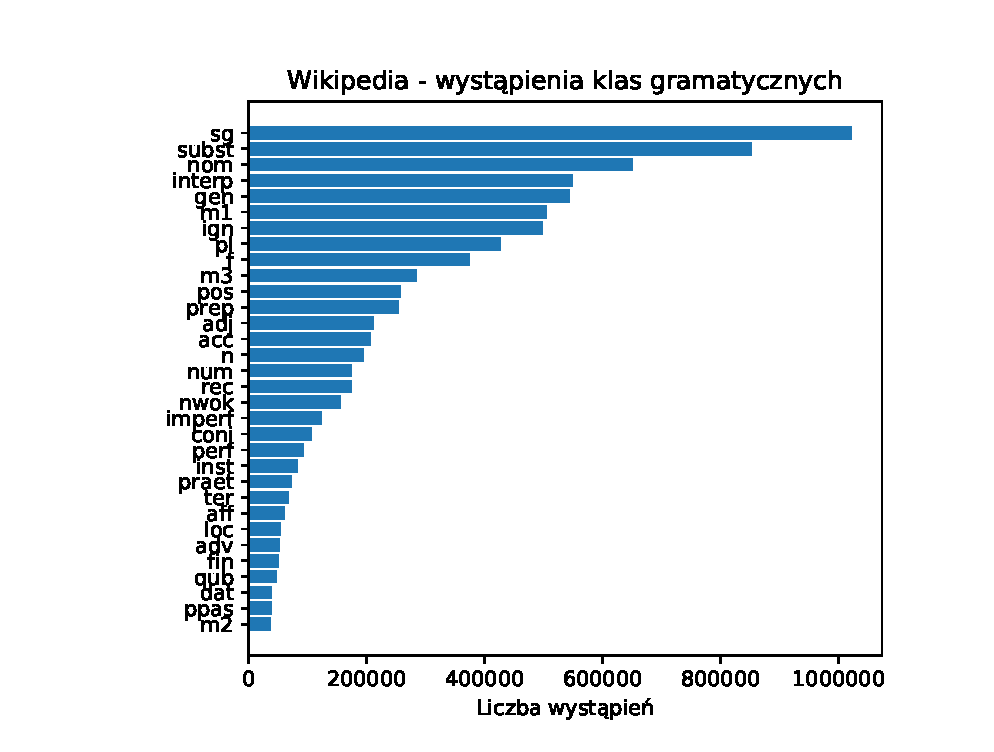
\includegraphics[width=0.8\linewidth]{img/gram-classes-wikipedia}}}
	\caption{Porównanie wystąpień klas gramatycznych w obu korpusach}
    \label{fig:corpus-ign}
\end{figure}

W przypadku korpusu \textit{Artykuły} nie rozpoznano około 5.19\% wyrazów w stosunku do całego korpusu. W korpusie \textit{Wikipedia} wartość ta wynosi tylko 1.12\%. Rozbieżności między tymi wartościami wynikają najprawdopodobniej z literówek, jakie mogły zaistnieć podczas pisania artykułów. W artykułach z platformy Wikipedia często są one poprawiane i redagowane przez więcej niż jedną osobę. 
W pełni automatyczna poprawa tekstu byłaby zadaniem trudnym; takie działanie mogłoby skutkować pogorszeniem wyników, jeśli słowo zostałoby nieprawidłowo zinterpretowane. W celu poprawy jakości zebranych danych, wyznaczone zostały najczęściej występujące nierozpoznane słowa zaprezentowane na rysunku \ref{fig:freq-ign-words}.

\begin{figure}[ht!]
	\centering
	\subfloat[Artykuły]{{\includegraphics[width=0.8\linewidth]{img/unknown-words-articles}}}
    \qquad
    \subfloat[Wikipedia]{{\includegraphics[width=0.8\linewidth]{img/unknown-words-wikipedia}}}
	\caption{Porównanie wystąpień nierozpoznanych form w obu korpusach}
    \label{fig:freq-ign-words}
\end{figure}

Formami nierozpoznanymi okazały się w głównej mierze nazwy własne. W obu korpusach są one częścią istotnych cech, które sugerują daną grupę tematyczną, dlatego pozostały w korpusach bez zmian. \textit{r} - prawdopodobnie jest to pozostałość po podziale wartości liczbowej roku oraz skrótu \textit{r.}.
Usunięto jedynie kilka wyrazów
\begin{itemize}
\item \textit{nbsp} (ang. non breaking space) - kod HTML dla spacji niełamliwej używanej w kodzie \cite{nbsp-wikipedia}
\item \textit{commons} oraz \textit{wikipedia} - od nazwy własnej Wikipedia Commons, prawdopodobnie błąd podczas pobierania
\end{itemize}

Należy jednak pamiętać, że klasyfikowane artykuły zawsze zawierać będą pewien odsetek tekstów, które są błędnie napisane. Dlatego zdecydowano się na usunięcie jedynie oczywistych błędów popełnionych podczas implementacji programów zbierających korpusy.

\subsection{Usunięcie wyrazów nierelewantnych}
Podczas analizy tekstu istotnym aspektem jest jakość analizowanych danych i dokumentów. W pracach dotyczących klasyfikacji tematycznej częstą praktyką jest usuwanie słów nierelewantnych w fazie przetwarzania  \cite{introInfoRetrieval}\cite{indeksowanietresci}\cite{mykowiecka}. Do słów nierelewantnych zalicza się wyrazy, które najczęściej występują w danym języku (ang. stop words). Dzięki temu współczynnikowi, jakość klasyfikacji ulega poprawie poprzez pomijanie mało istotnych wyrazów. Dodatkową zaletą jest mniejsze zapotrzebowanie na pamięć oraz moc obliczeniową, ponieważ przetwarzanych danych jest mniej. W pracy wykorzystano listę wyrazów, która została udostępniona na stronie \textit{https://www.ranks.nl/stopwords/polish} \cite{polishStopwords} w postaci tabeli.

\subsection{Analiza zawartości korpusu}
Kluczowym etapem okazała się ręczna analiza zawartości korpusu z wykorzystaniem takich metod jak modelowanie tematów (ang. topic modeling). Modelowanie tematów jest techniką analizy dużych zbiorów dokumentów; modele automatycznie wyszukują tematy w tekście z wykorzystaniem ukrytych zmiennych losowych. Technika ta często jest wykorzystywana do rekomendacji tagów, wyszukiwania słów kluczowych, kategoryzacji tekstów. \cite{about-lda} W pracy wykorzystano gotową implementację \textit{LDA} (Latent Allocation Dirichlet) z biblioteki \textit{SciKitLearn} w celu analizy zawartości zebranego korpusu. Wyniki analizy \ref{tab:lda-result} wykazały, że zawartość korpusu, mimo starannych prób usunięcia wszystkich wyrazów mogących powodować błędne wyniki, nie była idealna.



\begin{table}[ht!]
\centering
\caption{Wynik modelowania tematycznego przy pomocy LDA}
\label{tab:lda-result}
\begin{tabular}{|l|l|}
\hline
\multicolumn{1}{|c|}{Topic 0} & mecz rok polska 00 minuta pap pierwsza druga miejsce raz                       \\ \hline
Topic 1                       & urządzenie model smartfon móc sprzęt nowa ekran producent można wersja         \\ \hline
Topic 2                       & skóra kobieta móc należeć choroba woda często czas zabieg można                \\ \hline
Topic 3                       & samochód pojazd prezydent kierowca powiedzieć zostać ustawa złoty projekt auto \\ \hline
Topic 4                       & metr pkt polska konkurs niemcy pap stefan rok miejsce już pozycja seria        \\ \hline
Topic 5                       & niebezpiecznik dana serwer firma atak serwis móc sieć informacja błąd          \\ \hline
Topic 6                       & rok polski polska lato czas były państwo pap była wojna więc                   \\ \hline
\end{tabular}
\end{table}

W zawartości korpusu znalazły się słowa, które mogły dać klasyfikatorom jednoznaczne podpowiedzi, do której grupy przynależy tekst, na przykład \textit{pap} oraz \textit{niebezpiecznik}. W celu usunięcia niechcianych wyrazów dodano je do listy słów nierelewantnych. Analiza była przeprowadzana tak długo, dopóki wszystkie niechciane słowa nie zostały usunięte z wyników pracy \textit{LDA}. Ostatecznie zliczono wszystkie formy podstawowe wyrazów dla każdej kategorii i przedstawiono je na rysunku \ref{fig:rozklad-lemmatow-wg-zrodla}.

\begin{figure}[ht!]
	\centering
	\subfloat[Artykuły]{{\includegraphics[width=0.8\linewidth]{img/avg-lemma-count-articles}}}
    \qquad
    \subfloat[Wikipedia]{{\includegraphics[width=0.8\linewidth]{img/avg-lemma-count-wikipedia}}}
	\caption{Rozkład średniej liczby lematów według kategorii}
   \label{fig:rozklad-lemmatow-wg-zrodla}
\end{figure}
\newpage
\section{Metody klasyfikacji tekstu}
W pracy zdecydowano się na przetestowanie dwóch różnych metod klasyfikacji, \textit{Bag-Of-Words} oraz \textit{fastText}, który jest pochodną \textit{word2vec}.
\subsection{Bag-Of-Words}
Aby móc poddać tekst klasyfikacji, konieczne jest wstępne przetworzenie tekstu wejściowego i przedstawienie go w postaci macierzy lub, w przypadku prostszych metod, wektora wierszowego dla danego tekstu. Istnieje wiele różnych sposobów wektoryzacji dokumentów; najprostszym i najczęściej stosowanym \cite{BoulisText} jest model \textit{Bag-Of-Words}. Każdy dokument jest przedstawiany w postaci wektora wierszowego, który zawiera liczbę wystąpień słowa w danym dokumencie.\cite{joulin2016bag}
\subsubsection*{Przykład Bag-of-Words}
Utworzenie \textit{Bag-of-Words} na przykładzie dwóch dokumentów \cite{bow-example} wyglądałoby następująco: \\ \hfill
\begin{lstlisting}[style=someShit]
dokument 1: "The Sun is a star. Sun is beautiful."
dokument 2: "The Moon is a satellite."
\end{lstlisting}
Na podstawie zadanych dwóch dokumentów utworzony zostanie słownik z unikalnymi słowami. Liczba wszystkich unikalnych słów będzie również liczbą kolumn w każdym wektorze wierszowym dla całego korpusu dokumentów.\\

Przykładowe dokumenty składają się z 8 unikalnych słów, dlatego każdy dokument jest reprezentowany jako 8-elementowy wektor wierszowy i został przedstawiony na rysunku \ref{vectors-bow}.

\begin{table}[ht!]
\centering
\caption{Tabela wektorów Bag-Of-Words}
\label{vectors-bow}
\begin{tabular}{|l|c|c|}
\hline
\multicolumn{1}{|c|}{\textbf{słowo}} & \textbf{dokument 1} & \multicolumn{1}{l|}{\textbf{dokument 2}} \\ \hline
The                                                          & 1                   & 1                                                                \\ \hline
Sun                                                          & 2                   & 0                                                                \\ \hline
is                                                           & 2                   & 1                                                                \\ \hline
a                                                            & 1                   & 1                                                                \\ \hline
star                                                         & 1                   & 0                                                                \\ \hline
beautiful                                                    & 1                   & 0                                                                \\ \hline
Moon                                                         & 0                   & 1                                                                \\ \hline
satellite                                                    & 0                   & 1                                                                \\ \hline
\end{tabular}
\end{table}

Cyfra pierwsza '1' w obu dokumentach oznacz, że w dokumencie tylko raz wystąpiło słowo 'The'. Druga cyfra ('2') w dokumencie pierwszym oznacza, że słowo 'Sun' wystąpiło dwa razy, natomiast w dokumencie drugim ('0') ani razu nie pojawiło się słowo 'Sun'.
\begin{lstlisting}[caption=Utworzone wektory, style=someShit]
dokument 1: [1, 2, 2, 1, 1, 1, 0, 0]
dokument 2:  [1, 0, 1, 1, 0, 0, 1, 1]
\end{lstlisting}
\subsubsection*{Ustalenie wag - \textit{tf-idf}}
Algorytm \textit{tf-idf} służy do określania wag słów względem całego korpusu. Jeśli słowo pojawia się często we wszystkich dokumentach, jego znaczenie maleje, ponieważ prawdopodobnie nie wnosi ono żadnej praktycznej wiedzy. \textit{tf-idf} mierzy znaczenie, a nie częstotliwość i jego wartość jest obliczana według wzoru\cite{tfidf-eq}:

\begin{equation}
Wt,d = TFt,d log(N/DFt)
\end{equation}

Gdzie:
\begin{itemize}
\item $TFt,d$ - oznacza liczbę wystąpień słów $t$ w dokumentach $d$,
\item $DFt$ - oznacza liczbę dokumentów zawierających słowo $t$,
\item $N$ - oznacza liczbę wszystkich dokumentów w korpusie.
\end{itemize}

\subsubsection*{Implementacja Bag-Of-Words}
W pracy użyto narzędzia o nazwie \textit{CountVectorizer} z biblioteki \textit{SciKit Learn}, która służy do wyodrębniania cech numerycznych z treści tekstowej, a mianowicie\cite{skl-reference}:
\begin{itemize}
\setlength\itemsep{0.6em}
\item tokenizuje ciągi znaków, 
\item zlicza wystąpienia tokenów w każdym dokumencie,
\item usuwa \textit{stop words} z zadanej listy,
\item normalizuje i ustala wagi, liczbę próbek / liczbę dokumentów.
\end{itemize}

Tekstem wejściowym dla zastosowanego narzędzia \textit{CountVectorizer} były zlematyzowane teksty (hasła) uzyskane w fazie przetwarzania wstępnego. Kapitalizacja wszystkich wyrazów została usunięta i wszystkie litery zostały zamienione na małe. Efektem działania \textit{CountVectorizera} jest macierz terminów \textit{dokument} (ang. document-term), która opisuje częstotliwość występowania tokenów w zbiorze dokumentów. Kolumny odpowiadają kolejnym wyrazom, a wiersze dokumentom, tak jak przedstawiono w tabeli \ref{countvectorizer-output}.

\begin{table}[ht!]
\centering
\caption{Macierz dokument-wyrażenie}
\label{countvectorizer-output}
\begin{tabular}{|c|c|c|c|c|c|c|c|c|}
\hline
   & The & Sun & is & a & star & beautiful & Moon & satellite \\ \hline
D1 & 1   & 2   & 2  & 1 & 1    & 1         & 0    & 0         \\ \hline
D2 & 1   & 0   & 1  & 1 & 0    & 0         & 1    & 1         \\ \hline
\end{tabular}
\end{table}
\newpage
Końcową optymalizacją jest zastosowanie normalizacji \textit{tf-idf} w celu ustalenia wag lematów w macierzy. Tak przygotowana macierz może już być wprowadzona do klasyfikatora w celu nauki oraz późniejszych testów. Implementacja została zaprezentowana na listingu poniżej.

\begin{lstlisting}[style=pythonStyle]
#funkcja uruchamiajaca test BagOfWords
def invoke(
      data_train, data_test, #dane uczace
      target_train, target_test, #dane testowe
      clf, iterations): #klasyfikator, ilosc iteracji
    
    	#zmienne tymczasowe do wyznaczenia wartosci srednich
    fit_time_acc = 0 
    predict_time_acc = 0
    accuracy_acc = 0
    f1_acc = 0

	#petla iteracyjna
    for iter_index in range(0, iterations):
    	#wykonanie obliczen dla jednego kroku
        predicted, fit_time, predict_time = iter_step(
        	data_train, data_test, target_train, clf)
            
        #sumowanie obliocznych wynikow
        fit_time_acc += fit_time
        predict_time_acc += predict_time
        accuracy_acc += accuracy_score(target_test, predicted)
        f1_acc += f1_score(target_test, predicted, average='micro')

	#wyznaczenie wartosci srednich
    mean_fit_time = fit_time_acc / iterations
    mean_predict_time = predict_time_acc / iterations
    mean_accuracy = accuracy_acc / iterations
    mean_f1_acc = f1_acc / iterations

	#zwrocenie wynikow
    return mean_f1_acc, mean_accuracy, mean_fit_time, mean_predict_time


def iter_step(data_train, data_test, target_train, classifier):
	#pobranie listy slow nierelewatnych
    stop_words_list = read_stop_words_list("../data/stop_words/list.txt")
    countVectorizer = CountVectorizer(stop_words=stop_words_list)
    tfidf_vectorizer = TfidfVectorizer()
    
    	#stworzenie procesu
    pipeline = Pipeline([
    	('cnt', countVectorizer),
        ('vect', tfidf_vectorizer),
        ('clf', classifier)])

	#nauczenie wszystkich elementów w 'pipeline'
    start = time.time()
    pipeline = pipeline.fit(data_train, target_train)
    end = time.time()
    	#wyznaczenie czasu nauki
    fit_time = (end - start)

	#klasyfikacja danych testowych
    start = time.time()
    predicted = pipeline.predict(data_test)
    end = time.time()
    	#wyznaczenie czasu predykcji
    predict_time = (end - start)

	#zwrocenie wyników
    return predicted, fit_time, predict_time

\end{lstlisting}

\subsubsection{Badane klasyfikatory}
W pracy zdecydowano się na wykorzystanie trzech klasyfikatorów; do tego celu wybrano 3 najczęściej wykorzystywane klasyfikatory w pracach dotyczących klasyfikacji tematycznej. \cite{walkowiak2018} \cite{text-classification-stanford}\cite{maciej-baj}
\begin{itemize}
 \setlength\itemsep{2em}
\item \textbf{Wielomianowy naiwny klasyfikator bayesowski} (ang. Multinomial Naive Bayes) - metoda, która określa przynależność danego obiektu do klasy na podstawie prawdopodobieństwa. \cite{internet-stat-book} Klasyfikacja odbywa się przy wykorzystaniu cech z wartościami dyskretnymi (np. liczba słów dla klasyfikacji tekstu). Rozkład wielomianowy zwykle wymaga liczby elementów całkowitych. Jednak w praktyce mogą być to również liczby ułamkowe, występujące w przypadku wektoryzacji \textit{TF-IDF}. \cite{skl-reference}

\item \textbf{Liniowa maszyna wektorów nośnych} (ang. Linear Support Vector Machine) - SVM to zestaw nadzorowanych metod uczenia używanych do klasyfikacji. Metoda polega na wyznaczaniu granic hiperpłaszczyzny oddzielającej próbki każdej klasy. W pracy wykorzystano SVM z liniową funkcją separującą; oznacza to, że przestrzenie są tak dzielone, aby odległość pomiędzy każdym jej punktem, a najbliższym punktem innej płaszczyzny był jak największy. \cite{internet-stat-book}

\item \textbf{Drzewo decyzyjne} (ang. Decision Tree) - to nadzorowana metoda uczenia stosowana do klasyfikacji i regresji. Tworzony jest model, który jest w stanie klasyfikować dane poprzez naukę prostych reguł decyzyjnych wywnioskowanych z danych uczących. Im głębsze drzewo, tym bardziej złożone reguły decyzyjne. \cite{skl-reference}
\end{itemize}

\subsection{fastText}
\textit{fastText} to metoda klasyfikacji, stworzona w laboratorium AI Research (FAIR) w Facebooku jako projekt open-source, aby sprostać potrzebie zrozumienia znaczenia dużych zbiorów tekstów. Biblioteka została zaprojektowaną tak, aby ułatwić tworzenie skalowalnych rozwiązań do reprezentacji i klasyfikacji tekstu. Jest to stosunkowo nowa metoda wykorzystywana do kategoryzacji tekstu. W założeniu twórców ma ona umożliwiać klasyfikację bardzo dużych ilości danych w krótkim czasie przy niskich wymaganiach sprzętowych. Według autorów, \textit{fastText} potrafi klasyfikować 500 tysięcy zdań na 300 tysięcy kategorii w mniej niż 5 minut na zwykłych komputerach domowych. \cite{faster-better-fasttext}

\textit{FastText} wykorzystuje technikę osadzonych słów (ang. word embedding) i domyślnie używa klasyfikatora Softmax \cite{walkowiak2018}. Wykorzystuje także tablicę przeglądową (ang. lookup table) z haszowaniem dla n-gramów, składających się ze słów lub znaków. Każdy dokument reprezentowany jest jako średnia z osadzania słów. Zaletą tej metody jest zdolność do tworzenia wektorów dla dowolnych słów, nawet tych, które są niepoprawnie napisane (ponieważ w rzeczywistości wektory te zbudowane są z podłańcuchów znaków w nim zawartych). Dzięki temu, wektory mogą być budowane na podstawie złączonych ze sobą tylko dwóch słów. Istotną zaletą jest również zdecydowanie krótszy czas klasyfikacji oraz nauki w porównaniu do innych metod. Jest to rozszerzenie metody \textit{word2vec}, w której każde słowo w korpusie jest traktowane jako atomowa jednostka i generowany jest dla niej oddzielny wektor. \cite{joulin2016bag}  \textit{fastText} domyślnie ignoruje kolejność słów, podobnie jak metoda \textit{BoW}. Aby uwzględnić lokalną kolejność słów, \textit{fastText} pozwala na użycie n-gramów, jednak funkcja ta ostatecznie nie była używana w eksperymentach.\cite{joulin2016fasttext}



\subsubsection{Działanie word2vec}
Modele \textit{word2vec} oraz \textit{fastText} zostały stworzone przez zespół prowadzony przez Tomasa Mikolova z Google. Algorytm przyjmuje duży korpus tekstu jako wejście i tworzy przestrzeń wektorową, \cite{nlp-from-scratch} zazwyczaj o kilkuset wymiarach z każdym unikalnym wyrazem w korpusie, któremu przypisuje odpowiedni wektor w przestrzeni. Wektory słów są umieszczane w przestrzeni wektorowej w taki sposób, że słowa, które mają wspólne konteksty w korpusie, znajdują się blisko siebie w przestrzeni. Przykład takich relacji został zaprezentowany na rysunku \ref{fig:word2vec-relation}. \cite{word2vec-google}

\begin{figure}[ht!]
	\centering
	\fbox{\includegraphics[width=1\linewidth]{img/linear-relationships}}
	\caption{Liniowa zależność word2vec}
	\label{fig:word2vec-relation}
\end{figure}

\subsubsection{Implementacja Python}
Biblioteka \textit{fastText} została oryginalnie napisana w języku C++ i nie ma dostępnych żadnych oficjalnych \textit{wrapperów} do języka Python. Jednak w sieci istnieje wiele rozwiązań, które pozwalają na wykorzystanie \textit{fastText} w języku Python. W pracy wykorzystano wrapper o nazwie \textit{ShallowLearn} (więcej informacji \url{https://github.com/giacbrd/ShallowLearn}), który jest zbiorem modeli uczenia opartym na płytkich podejściach do sieci neuronowych (np. \textit{word2vec} i \textit{fastText}). Do wykorzystanego wrappera należało również stworzyć odpowiedni adapter, który realizował funkcję konwertera danych wejściowych do oczekiwanego przez wrapper format. Dodatkowo otrzymywane przez \textit{ShallowLearn} wyniki musiały zostać poddane odpowiedniemu przetworzeniu tak, aby dane wyjściowe były reprezentowane w takiej samej postaci, jak ma to miejsce w przypadku implementacji \textit{Bag-Of-Words}. W tym celu stworzona została klasa \textit{calc\_adaper.py}, która poprawiała kompatybilność z biblioteką \textit{SciKit-Learn}. Możliwe stało się wykorzystanie metod dostarczanych przez interfejs biblioteki, \textit{fit} oraz \textit{predict}.
\chapter{Badanie skuteczności metod}
Wszystkie testy zostały przeprowadzone 10 razy z tymi samymi parametrami lecz za każdym razem z nowo wylosowanymi dokumentami, poddanymi wcześniej fazom przetwarzania, lematyzacji, wektoryzacji, a następnie klasyfikacji. Wyniki z iteracji tych samych testów zostały uśrednione i przedstawione na wykresach. 

\section{Korpus porównawczy}
Do celów porównawczych wykorzystano dodatkowo korpus o nazwie \textit{Wiki train - 34 categories}, dostępny w repozytorium Clarin \cite{11321/222}. Składa się on z 6800 dokumentów podzielonych na 34 klasy. Został on poddany tym samym procesom przetwarzania, co zebrany korpus z artykułami. Poszczególne kroki przetwarzania zostały pokazane na rysunku \ref{fig:process-flow}.

\begin{figure}[ht!]
	\centering
	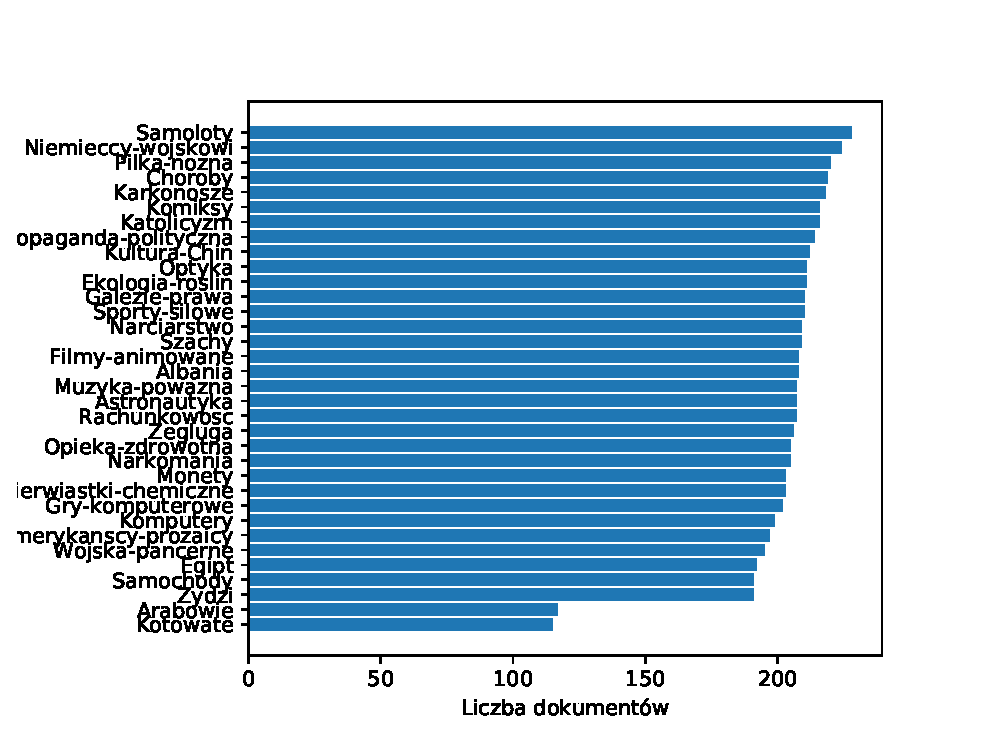
\includegraphics[width=0.8\linewidth]{img/count-files-wikipedia}
	\caption{Porównanie ilości dokumentów dla każdej klasy dla korpusu Wikipedii}
\end{figure}

\newpage
\section{Badane parametry}

Do określenia jakości wykorzystano cztery różne powszechnie stosowane parametry miar jakościowych \cite{walkowiak2018} \cite{maciej-baj}. Dodatkowo zmierzony został czas pracy każdego z klasyfikatorów nad różnymi etapami pracy.



\begin{itemize}
 \setlength\itemsep{2em}
\item \textbf{czułość} (ang. recall) - jest liczbą poprawnych pozytywnych wyników podzieloną przez liczbę wszystkich odpowiednich próbek (wszystkie próbki, które powinny zostać zidentyfikowane jako pozytywne). \cite{skl-reference} Czułość określa się wzorem:

\begin{equation}
\label{recallEq}
R = \frac{T_{p}}{T_{p} + F_{n}}
\end{equation}
Gdzie:
\begin{itemize}
\item $T_{p}$ - oznacza liczbę poprawnie rozpoznanych dokumentów
\item $F_{n}$ - oznacza liczbę niepoprawnie nierozpoznanych dokumentów
\end{itemize}

\item \textbf{precyzja} (ang. precision) - jest liczbą poprawnych pozytywnych wyników podzieloną przez liczbę wszystkich pozytywnych wyników zwróconych przez klasyfikator. \cite{skl-reference} Precyzję określa się wzorem:

\begin{equation}
\label{precisionEq}
P = \frac{T_{p}}{T_{p} + F_{p}}
\end{equation}
Gdzie:
\begin{itemize}
\item $T_{p}$ - oznacza liczbę poprawnie rozpoznanych dokumentów
\item $F_{p}$ - oznacza liczbę niepoprawnie rozpoznanych dokumentów
\end{itemize}

\item \textbf{miara f1} (ang. f1-score) - w statystycznej analizie klasyfikacji jest to miara dokładności testu. Uwzględnia ona dwa wcześniejsze parametry: precyzję oraz czułość. Jest średnią harmoniczną, gdzie wynik F1 osiąga najwyższą wartość 1 (doskonała precyzja i czułość), a najgorszy - 0. \cite{miary-jakosci}

\begin{equation}
F1 = 2*\frac{P * R}{P+R}
\end{equation}

Gdzie:
\begin{itemize}
\item $P$ - oznacza precyzję opisywaną we wzorze \ref{precisionEq}
\item $R$ - oznacza czułość opisywaną we wzorze \ref{recallEq}
\end{itemize}

\item \textbf{dokładność} (ang. accuracy) - stosunek między poprawnie sklasyfikowanymi dokumentami do wszystkich dokumentów. \cite{skl-reference}

\begin{equation}
A = \frac{T_{p} + T_{n}}{T_{p} + T_{n} + F_{p} + F_{n}}
\end{equation}

Gdzie:
\begin{itemize}
\item $T_{p}$ - oznacza liczbę poprawnie rozpoznanych dokumentów
\item $T_{n}$ - oznacza liczbę poprawnie nierozpoznanych dokumentów
\item $F_{p}$ - oznacza liczbę niepoprawnie rozpoznanych dokumentów
\item $F_{n}$ - oznacza liczbę niepoprawnie nierozpoznanych dokumentów
\end{itemize}
\end{itemize}


Dodatkowo w testach uwzględniono inne miary niż jakościowe, a mianowicie:
\begin{itemize}
\item \textbf{czas nauki klasyfikatora} - czas wyrażony w sekundach, potrzebny systemowi na naukę danego klasyfikatora danymi wejściowymi. Ściślej mówiąc, jest to czas potrzebny na wykonanie się metod; był odpowiedzialny za nauczenie modelu dla każdego użytego klasyfikatora. 

\item \textbf{czas klasyfikacji} - czas wyrażony w sekundach, potrzebny systemowi na klasyfikację zbioru dokumentów. 

\item \textbf{całkowity czas pracy} - czas wyrażony w sekundach, jest to suma czasu potrzebnego na naukę oraz klasyfikację zbioru dokumentów.
\end{itemize}

\section{Wyniki testów}

Całość badanego korpusu z artykułami składała się z 2600 artykułów, podzielonych na 7 klas, po 380 dokumentów dla każdej kategorii. Szczegółowe informacje dotyczące wykorzystanych korpusów przedstawiono w tabeli \ref{fig:korpus-compare}. Z tego zbioru część artykułów przeznaczono do trenowania oraz część do testowania. W przypadku krzywej nauczania, wszystkie artykuły brały udział w teście. Ilość danych testowych była uzależniona od liczby danych uczących i była liczbą, która pozostała po odjęciu liczby dokumentów niebiorących udziału w fazie nauczania. Badania rozpoczęto od próby dopasowania optymalnych parametrów dla danego zbioru danych. Z obu pełnych korpusów zostały wyznaczone dwa dodatkowe, zawierające jedynie formy podstawowe rzeczowników, sklasyfikowane przy pomocy analizatora WCRTF2 podczas przetwarzania wstępnego. Taki korpus został podpisany hasłem \textit{rzeczowniki}.

\begin{table}[ht!]
\centering
\caption{Porównanie badanych korpusów danych}
\label{fig:korpus-compare}
\begin{tabular}{|l|l|l|l|l|}
\hline
nazwa korpusu & l. dokumentów & l. klas & l. dokumentów na klasę & rozmiar na dysku \\ \hline
Wikipedia     & $\sim$6800        & 34         & $\sim$200 & 34MB               \\ \hline
Artykuły      & $\sim$2600        & 7          & $\sim$380  & 12MB              \\ \hline
Wikipedia (rzeczowniki)     & $\sim$6800        & 34         & $\sim$200 & 28MB               \\ \hline
Artykuły (rzeczowniki)     & $\sim$2600        & 7          & $\sim$380 & 8.6MB               \\ \hline
\end{tabular}
\end{table}

\subsection{Bag-Of-Words}

W modelu \textit{Bag-Of-Words} w każdym teście została domyślnie użyta normalizacja \textit{tf-idf} z listą słów nierelewantnych. Zmieniany był parametr n-gram oraz rodzaj zawartości n-gramów. Przetestowano dwa różne scenariusze:
\begin{itemize}
\item Scenariusz 1: analiza słów n-gramowych dla wartości parametru \textit{n-gram}: 1, 2, 3
\item Scenariusz 2: analiza znaków n-gramowych dla wartości parametru \textit{n-gram}: 5, 6, 7
\end{itemize}
Testy zostały przeprowadzone z wykorzystaniem trzech klasyfikatorów (NaiveBayes, SVM, drzewo decyzyjne) a wyniki zostały uśrednione w celu zwiększenia czytelność wykresów oraz opisane pod wspólną nazwą \textit{BoW} na wykresach. Scenariusze zostały przetestowane dla obydwu wykorzystywanych w pracy korpusów.

W przypadku analizy znaków, lista \textit{stop words} nie była wykorzystywana i żadne słowa nie zostały odrzucone. 

\begin{figure}[ht!]
	\centering
	\subfloat[Artykuły]{{\includegraphics[width=0.45\linewidth]{img/bag-of-words-tfidf-articles-words-n-gram}}}
    \qquad
    \subfloat[Wikipedia]{{\includegraphics[width=0.45\linewidth]{img/bag-of-words-tfidf-wikipedia-words-n-gram}}}
	\caption{Porównanie dokładności klasyfikacji \textit{Bag-Of-Word} dla n-gramów składających się ze słów - Scenariusz 1}
    \label{fig:bow-ngram-compare-word}
\end{figure}

W pierwszym testowanym scenariuszu \ref{fig:bow-ngram-compare-word} dokładność klasyfikacji była niższa dla większych wartości \textit{n-gram}, co jest zgodne z intuicją. Większa ilość słów wchodzących w skład n-gramu, w przypadku niewielkiej ilości danych, zwraca niższe rezultaty; jest to spowodowane większą trudnością odnalezienia i dopasowania takiego samego n-gramu. Wykres \ref{fig:bow-ngram-compare-word} pokazuje, że bigramy oraz unigramy uzyskały ostatecznie zbliżone wyniki. Wynika to prawdopodobnie z faktu, iż liczba klas była mniejsza, przez co pojawiało się zdecydowanie mniej unikalnych słów w korpusie. 

\begin{figure}[ht!]
	\centering
	\subfloat[Artykuły]{{\includegraphics[width=0.45\linewidth]{img/bag-of-words-tfidf-articles-char-n-gram}}}
    \qquad
    \subfloat[Wikipedia]{{\includegraphics[width=0.45\linewidth]{img/bag-of-words-tfidf-wikipedia-char-n-gram}}}
	\caption{Porównanie dokładności klasyfikacji \textit{Bag-Of-Word} dla n-gramów składających się ze znaków - Scenariusz 2}
    \label{fig:bow-ngram-compare-char}
\end{figure}

W drugim testowanym scenariuszu nie stwierdzono większych różnic pomiędzy użytymi wartościami parametrów. Wyniki końcowe wykazały, że użycie n-gramów składających się ze słów, w tym przypadku zwraca lepsze wyniki niż użycie n-gramów składających się ze znaków. Wyniki końcowe z najlepszymi uzyskanymi wartościami dokładności i odpowiadającym im parametrom przedstawiono w tabeli \ref{tab:bow-scenario-results}.

\begin{table}[]
\centering
\caption{Najlepsze wyniki testów \textit{Bag-Of-Words} dla różnych wartości n-gram i rodzaju analizowanych n-gramów}
\label{tab:bow-scenario-results}
\begin{tabular}{|l|c|c|c|}
\hline
scenariusz & nazwa korpusu                         & n-gram & dokładność \\ \hline
Scenariusz 1                     & Artykuły                       & 1 (słowa)     & 0.92                            \\ \hline
Scenariusz 1                     & Wikipedia & 1 (słowa)     & 0.82                            \\ \hline
Scenariusz 2                     & Artykuły  & 7 (znaki)      & 0.96                            \\ \hline
Scenariusz 2                     & Wikipedia                      & 5 (znaki)      & 0.82                            \\ \hline
\end{tabular}
\end{table}


Użycie modelu \textit{n-gramowego} dla znaków mogłoby zwracać lepsze rezultaty w przypadku dużej liczby słów, których analizatory morfologiczne nie były w stanie poprawnie rozpoznać i sprowadzić do ich form podstawowych. Przykładem mogłaby być sytuacja, kiedy w tekście znajduje się duża liczba literówek - uniemożliwiłoby to poprawne porównanie dwóch takich samych słów jednak napisanych z błędami.

\subsection{fastText}
Biblioteka \textit{fastText} według założeń przyjmuje zbiory dokumentów, bez żadnych modyfikacji. \cite{joulin2016fasttext} W pracy podjęto próbę optymalizacji tej metody, mającą na celu zmniejszenie czasu pracy bez wpływu na jakość wyników. W celu ograniczenia zbioru dokumentów wejściowych dla \textit{fastText}, zostały one poddane takiemu samemu procesowi jak w metodzie \textit{BoW}; proces ten został przedstawiony na rysunku \ref{fig:process-flow}. W celu wyboru optymalnych parametrów dla zmodyfikowanych korpusów wejściowych, przetestowano zmianę każdego z parametrów przy pozostawieniu domyślnych parametrów dla pozostałych wartości. Za najlepszą wartość parametru przyjmowano tą, przy użyciu której ostatecznie zwracane były najwyższe wyniki dla miary dokładności. Rezultaty przy użyciu zmienionych parametrów zostały zaznaczone na wykresach jako \textit{fastText (zmodyfikowany)}\footnote{W dalszej części pracy \textit{fastText (zmodyfikowany)} jest również zamiennie określany jako \textit{fastText}.}. Wyniki zostały uśrednione po 10 przebiegach dla każdego testu.


\subsubsection{Zmiana parametru \textit{ngram}}


\begin{figure}[ht!]
	\centering    
    \subfloat[Artykuły]{{\includegraphics[width=0.45\linewidth]{img/fasttext-ngram-articles}}}
    \qquad
    \subfloat[Artykuły (rzeczowniki)]{{\includegraphics[width=0.45\linewidth]{img/fasttext-ngram-articles-nouns}}}
    
    \subfloat[Wikipedia]{{\includegraphics[width=0.45\linewidth]{img/fasttext-ngram-wikipedia}}}
    \qquad
    \subfloat[Wikipedia (rzeczowniki)]{{\includegraphics[width=0.45\linewidth]{img/fasttext-ngram-wikipedia-nouns}}}
    
	\caption{Porównanie wyników zmiany parametru \textit{n-gram}}
    \label{fig:fasttext-ngram}
\end{figure}


Parametr \textit{ngram} określa maksymalną długość na jaką zostanie podzielony zbiór wyrazów.
Wszystkie trzy instancje w początkowej fazie osiągnęły podobny wynik dokładności, kolejne iteracje wskazały że instancja z parametrem \textit{ngram=1} uczyła się najszybciej i to ona ostatecznie osiągnęła też najlepsze wyniki, dla wszystkich czterech przypadków. Jest to skutek odwrotny do oczekiwanego, w żadnym momencie \textit{fastText} z użyciem bigramów nie osiągnął lepszego wyniku niż unigramy \cite{joulin2016bag}. Powodem takich rezultatów jest prawdopodobnie fakt, iż w przypadku korpusu z artykułami bardziej informacyjne były unigramy niż formy zawierające więcej n-gramów. Wyniki zostały przedstawione na rysunku \ref{fig:fasttext-ngram}.

\subsubsection{Zmiana parametru \textit{min\_count}}
Parametr \textit{min\_count} odrzuca wyrazy, które występują częściej niż zadana wartość, wyniki zmiany parametru zaprezentowano na rysunku \ref{fig:fasttext-mincount}.



\begin{figure}[ht!]
	\centering    
    \subfloat[Artykuły]{{\includegraphics[width=0.45\linewidth]{img/fasttext-min_count-articles}}}
    \qquad
    \subfloat[Artykuły (rzeczowniki)]{{\includegraphics[width=0.45\linewidth]{img/fasttext-min_count-articles-nouns}}}
    
    \subfloat[Wikipedia]{{\includegraphics[width=0.45\linewidth]{img/fasttext-min_count-wikipedia}}}
    \qquad
    \subfloat[Wikipedia (rzeczowniki)]{{\includegraphics[width=0.45\linewidth]{img/fasttext-min_count-wikipedia-nouns}}}
    
	\caption{Porównanie wyników zmiany parametru \textit{min\_count}}
    \label{fig:fasttext-mincount}
\end{figure}

Wyniki dla 5 testowanych wartości zbiegają do tego samego poziomu. Najwięcej próbek potrzebował algorytm w przypadku parametru \textit{min\_count=100}. Początkowe wyniki na przedstawionych rysunkach \ref{fig:fasttext-mincount} wyraźnie pokazują, że najlepszą wartością w tym przypadku jest wartość 20. Dla korpusów z rzeczownikami można zaobserwować zmniejszenie się różnic w wynikach jakościowych pomiędzy wartościami: 0, 5, 10 oraz 20.
\newpage
\subsubsection{Zmiana parametru \textit{loss}}
Do wyboru są trzy różne wartości, które definiują który klasyfikator zostanie użyty podczas pracy. Domyślnym klasyfikatorem dla \textit{fastText} jest \textit{softmax} \cite{walkowiak2018}.

\begin{figure}[ht!]
	\centering    
    \subfloat[Artykuły]{{\includegraphics[width=0.45\linewidth]{img/fasttext-loss-articles}}}
    \qquad
    \subfloat[Artykuły (rzeczowniki)]{{\includegraphics[width=0.45\linewidth]{img/fasttext-loss-articles-nouns}}}
    
    \subfloat[Wikipedia]{{\includegraphics[width=0.45\linewidth]{img/fasttext-loss-wikipedia}}}
    \qquad
    \subfloat[Wikipedia (rzeczowniki)]{{\includegraphics[width=0.45\linewidth]{img/fasttext-loss-wikipedia-nouns}}}
    
	\caption{Porównanie wyników zmiany parametru \textit{loss}}
    \label{fig:fasttext-loss}
\end{figure}

Zmiana parametru \textit{loss} nie powodowała tak dużych zmian w wynikach jak poprzednie parametry. Jednoznacznie jednak można stwierdzić, że przy mniejszej ilości próbek algorytm \textit{softmax} zwraca lepsze wyniki niż pozostałe dwie metody. Ostatecznie najlepsze wyniki w przypadku użytego korpusu osiągnięto przy pomocy algorytmu \textit{ns (negative samples)} i to on zostanie użyty w końcowych testach porównawczych. Wyniki na wykresach zostały przedstawione na rysunku \ref{fig:fasttext-loss}.

\newpage
\subsubsection{Zmiana parametru \textit{epoch}}

Parametr \textit{epoch} oznacza liczbę iteracji, które musi wykonać algorytm, aby nauczyć się korpusu \cite{fasttext-github}. Liczba iteracji jest tożsama z liczbą możliwości zobaczenia przez \textit{fastText} konkretnego dokumentu. 

\begin{figure}[ht!]
	\centering    
    \subfloat[Artykuły]{{\includegraphics[width=0.45\linewidth]{img/fasttext-epoch-articles}}}
    \qquad
    \subfloat[Artykuły (rzeczowniki)]{{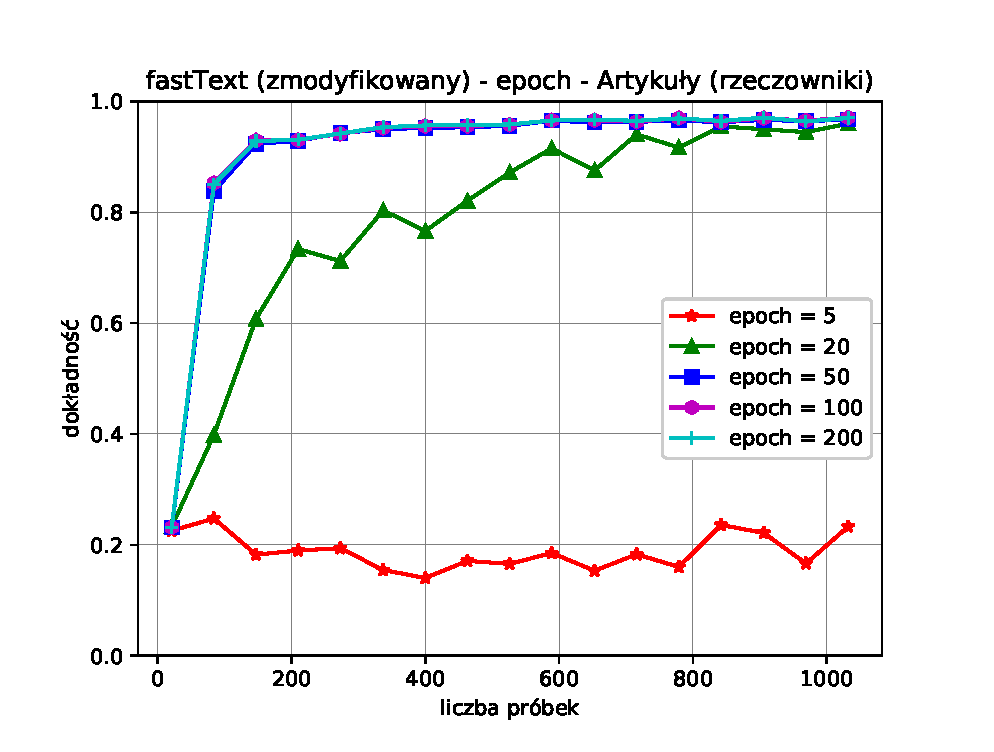
\includegraphics[width=0.45\linewidth]{img/fasttext-epoch-articles-nouns}}}
    
    \subfloat[Wikipedia]{{\includegraphics[width=0.45\linewidth]{img/fasttext-epoch-wikipedia}}}
    \qquad
    \subfloat[Wikipedia (rzeczowniki)]{{\includegraphics[width=0.45\linewidth]{img/fasttext-epoch-wikipedia-nouns}}}
    
	\caption{Porównanie wyników zmiany parametru \textit{epoch}}
    \label{fig:fasttext-epoch}
\end{figure}

Domyślną wartością parametru \textit{epoch} w \textit{fastText} jest wartość 5 i w przypadku wykorzystanych korpusów zwracane wyniki są bardzo niskie, niezależnie od ilości próbek. Najlepsze wyniki osiągnięto przy użyciu wyższych wartości, kosztem czego jest dłuższy czas nauki algorytmu, co jest oczekiwanym efektem. Wartości 50, 100 oraz 200 uzyskują zbliżone do siebie wyniki w przypadku korpusu z rzeczownikami, z widoczną korzyścią dla wartości 200 w pełnym korpusie. Wartości pośrednie - 50 oraz 20, wraz ze zwiększającą ilością danych testowych dąży do wyników osiąganych przez najlepsze wartości parametrów.

\subsubsection{Zmodyfikowane parametry}
Ostatecznie dobrano optymalne wartości dla każdego parametru i  przedstawiono je w tabeli \ref{tab:optimal-param}. Kolejne testy wykonano przy ich użyciu, a metodę określano jako \textit{fastText (zmodyfikowany)}.

\begin{table}[hb!]
\centering
\caption{Optymalne parametry biblioteki \textit{fastText} dla testowanych danych}
\label{tab:optimal-param}
\begin{tabular}{|c|c|c|c|}
\hline
ngram & min\_count & loss                  & epoch \\ \hline
1     & 20         & ns (negative samples) & 200   \\ \hline
\end{tabular}
\end{table}

\clearpage
\section{Porównanie wyników}

Podczas wyznaczania raportów jakości, dane treningowe stanowiły stosunek 70 do 30 dla obu testowanych korpusów. Składały się z 1820 dokumentów uczących oraz 780 dokumentów testujących, co stanowiło stosunek 70 do 30.
%%%%%%%%%%%%%%%%%%%%%%%%%%%%%%%%%%%%%%%%%%%%%%%%%%%%%%%%%%%%%%%%%%%%%%%%%%%%%%%%%%%%%%%%%%%%%%%%%%%%

\subsection{Analiza zbadanych miar}
Dla każdego klasyfikatora wygenerowana została tabela z wynikami miar dla każdej klasy w zbiorze dokumentów: \textit{precyzji (ang. precision)}, \textit{czułości (ang. recall)}, \textit{miary f1 (ang. f1-score)}. W ostatnim wierszu znajdują się wartości uśrednione oznaczone jako \textit{średnia}.


%%%%%%%%%%%%%%%%%%%%%%%%%%%%%%%%% NB
\subsubsection{Naive Bayes}
\begin{figure}[ht!]
	\centering
	\subfloat[Artykuły]{{\includegraphics[width=0.45\linewidth]{img/report-naivebayes-articles}}}
    \qquad
    \subfloat[Artykuły (rzeczowniki)]{{\includegraphics[width=0.45\linewidth]{img/report-naivebayes-articles-nouns}}}
	\caption{Miary jakościowe - NaiveBayes - Artykuły}
    \label{fig:report-naivebayes-articles}
\end{figure}
Rysunek \ref{fig:report-naivebayes-articles} przedstawia porównanie zbadanych miar dla pełnego korpusu oraz korpusu z samymi rzeczownikami. Według analizy skuteczność klasyfikatora \textit{NaiveBayes} w obu przypadkach jest zbliżona do siebie. Pojawiają się minimalne różnice na korzyść pełnych korpusów, co można zaobserwować w przypadku klasy \textit{zdrowie} oraz \textit{sprzęt}. Średnie wartości były takie same.

\begin{figure}[ht!]
	\centering
	\subfloat[Wikipedia]{{\includegraphics[width=0.45\linewidth]{img/report-naivebayes-wikipedia}}}
    \qquad
    \subfloat[Wikipedia (rzeczowniki)]{{\includegraphics[width=0.45\linewidth]{img/report-naivebayes-wikipedia-nouns}}}
	\caption{Miary jakościowe - NaiveBayes - Wikipedia}
    \label{fig:report-naivebayes-wikipedia}
\end{figure}

Rysunek \ref{fig:report-naivebayes-wikipedia} przedstawia analogiczne porównanie zbiorów dla 34 klasowego korpusu Wikipedii. Średnie wyniki wskazują na to, że różnice pogłębiły się lecz wciąż były one bardzo małe. Wyniki miary f1 zostały bez zmian. Warto również zauważyć, że dla niektórych klas uzyskano lepsze wyniki; dobrym przykładem jest klasa \textit{propaganda-polityczna}, której wynik miary f1 poprawił się o 10 punktów procentowych w stosunku do pełnego korpusu. Mimo braku zmiany średniej wartości miary f1 widać poprawę w większości klas, które były słabo rozpoznawane. Wyjątkiem od reguły jest klasa \textit{kultura-chin}, której wynik czułości spadł o 4 punkty procentowe.

%%%%%%%%%%%%%%%%%%%%%%%%%%%%%%%%% SVM
\subsubsection{SVM}
\textit{SVM} uzyskał bardzo dobre wyniki we wszystkich przypadkach. Średnie wartości były najwyższe dla każdego typu testowanych danych dla badanych klasyfikatorów. 
\begin{figure}[ht!]
	\centering
	\subfloat[Artykuły]{{\includegraphics[width=0.45\linewidth]{img/report-svm-articles}}}
    \qquad
    \subfloat[Artykuły (rzeczowniki)]{{\includegraphics[width=0.45\linewidth]{img/report-svm-articles-nouns}}}
	\caption{Miary jakościowe - SVM - Artykuły}
    \label{fig:report-svm-articles}
\end{figure}

Wykresy na rysunku \ref{fig:report-svm-articles} jednoznacznie wskazują na bardzo dobre dopasowania każdej z klas. Najniższa zanotowana wartość miary była nie niższa niż 0.96; klasyfikator \textit{SVM} niemal bezbłędnie rozpoznawał wszystkie klasy. Dla tych dwóch zbiorów ocena, czy użycie samych rzeczowników pozytywnie wpływa na jakość klasyfikacji, byłaby nadinterpretacją lecz z całą pewnością można stwierdzić, że nie ma negatywnego wpływu na przypisywanie kategorii zadanym tekstom.  

\begin{figure}[ht!]
	\centering
	\subfloat[Wikipedia]{{\includegraphics[width=0.45\linewidth]{img/report-svm-wikipedia}}}
    \qquad
    \subfloat[Wikipedia (rzeczowniki)]{{\includegraphics[width=0.45\linewidth]{img/report-svm-wikipedia-nouns}}}
	\caption{Miary jakościowe - SVM - Wikipedia}
    \label{fig:report-svm-wikipedia}
\end{figure}

Bardziej precyzyjne wnioski można otrzymać dopiero po analizie wyników na rysunku \ref{fig:report-svm-wikipedia}. Większa liczba klas wystarczająco utrudniła dopasowywanie kategorii, można zaobserwować, że średnie wyniki wszystkich rozpatrywanych miar pogorszyły się o 1/2 punkty procentowe. Słabo rozpoznawane kategorie z przedziału od 0.7 do 0.8 nie były lepiej dopasowywane w zbiorze dokumentów z samymi rzeczownikami.   

%%%%%%%%%%%%%%%%%%%%%%%%%%%%%%%%% DT 

\subsubsection{Drzewo decyzyjne}
\textit{Drzewo decyzyjne} osiągało najgorsze wyniki, ze wszystkich testowanych klasyfikatorów dla badanych zbiorów danych.
\begin{figure}[ht!]
	\centering
	\subfloat[Artykuły]{{\includegraphics[width=0.45\linewidth]{img/report-decisiontree-articles}}}
    \qquad
    \subfloat[Artykuły (rzeczowniki)]{{\includegraphics[width=0.45\linewidth]{img/report-decisiontree-articles-nouns}}}
	\caption{Miary jakościowe - Drzewo decyzyjne - Artykuły}
    \label{fig:report-dt-articles}
\end{figure}

Wszystkie kategorie uzyskały gorsze wyniki dla miary f1 po odrzuceniu innych części mowy niż rzeczowniki, o czym również świadczą niższe wartości średnie. Wysokie wskaźniki dla klasy \textit{sprzęt} są wynikiem bardzo charakterystycznych zbiorów słów występujących w tej kategorii, bowiem zawiera ona bardzo dużo nazw własnych, co zostało zobrazowane na rysunku \ref{fig:freq-ign-words}.

\begin{figure}[ht!]
	\centering
	\subfloat[Wikipedia]{{\includegraphics[width=0.45\linewidth]{img/report-decisiontree-wikipedia}}}
    \qquad
    \subfloat[Wikipedia (rzeczowniki)]{{\includegraphics[width=0.45\linewidth]{img/report-decisiontree-wikipedia-nouns}}}
	\caption{Miary jakościowe - Drzewo decyzyjne - Wikipedia}
    \label{fig:report-dt-wikipedia}
\end{figure}

Ważnym wnioskiem po analizie rysunku \ref{fig:report-dt-wikipedia} jest fakt iż, klasyfikacja dla korpusu z rzeczownikami w większości pogłębiła różnice między korpusami. Słabe wyniki, poniżej wartości 0.7 miary f1, obniżyły się, a wysokie wyniki, powyżej 0.8, polepszyły. Przykładami takiego zachowania są klasy \textit{karkonosze} (polepszenie), \textit{żydzi} (pogorszenie), \textit{propaganda-polityczna} (pogorszenie), \textit{gałęzie-prawa} (pogorszenie)



%%%%%%%%%%%%%%%%%%%%%%%%%%%%%%%%% fastText
\clearpage
\subsubsection{fastText}
\textit{fastText} osiągał wyniki zbliżone do tych, które zwracały klasyfikatory \textit{NaiveBayes} oraz \textit{SVM}, co plasuje go na drugim miejscu pod względem jakości dopasowywanych klas na podstawie otrzymanych średnich wyników dla testowanych miar na badanych korpusach.  
\begin{figure}[ht!]
	\centering
	\subfloat[Artykuły]{{\includegraphics[width=0.45\linewidth]{img/report-fasttext-articles}}}
    \qquad
    \subfloat[Artykuły (rzeczowniki)]{{\includegraphics[width=0.45\linewidth]{img/report-fasttext-articles-nouns}}}
	\caption{Miary jakościowe - fastText - Artykuły}
    \label{fig:report-fasttext-articles}
\end{figure}

\textit{fastText} bardzo dobrze klasyfikował artykuły w obu przypadkach, co pokazuje rysunek \ref{fig:report-fasttext-articles}. Nie utracił on znacznie skuteczności w jakości działania, mimo ograniczania zbioru dokumentów do samych rzeczowników. 

\begin{figure}[ht!]
	\centering
	\subfloat[Wikipedia]{{\includegraphics[width=0.45\linewidth]{img/report-fasttext-wikipedia}}}
    \qquad
    \subfloat[Wikipedia (rzeczowniki)]{{\includegraphics[width=0.45\linewidth]{img/report-fasttext-wikipedia-nouns}}}
	\caption{Miary jakościowe - fastText - Wikipedia}
    \label{fig:report-fasttext-wikipedia}
\end{figure}

Pełniejszy obraz dało przebadanie klasyfikatora na zbiorze danych z większą liczbą klas. Podobnie jak w pozostałych przypadkach, końcowe wartości średnie nieznacznie obniżyły się, co można uznać za regułę niezależnie od ilości danych i rodzaju użytego klasyfikatora badanego w pracy.

\subsubsection{Wnioski}
Na podstawie przebadanych klasyfikatorów i analizie badanych miar, podstawowym wnioskiem jaki należy wysnuć jest fakt, iż w każdym przypadku jakość klasyfikacji nieznacznie obniża się o około kilka punktów procentowych dla wszystkich miar lub pozostaje bez zmian. Jest to oczekiwany wynik \cite{walkowiak2018} obniżenia się jakości wyników. 
Bardzo niskie wartości miar dla drzewa decyzyjnego w stosunku do innych klasyfikatorów pozwoliły na stwierdzenie pewnej zależności między pełnym korpusem, a korpusem z rzeczownikami. W wielu przypadkach, gdzie dopasowanie klasy w pełnym korpusie jest niskie, widać pogorszenie się tego wyniku dla samych rzeczowników. Natomiast jeśli wartość miary f1 jest wysoka dla pełnego korpusu, wynik będzie wyższy dla samych rzeczowników. Reguła ta najbardziej widoczna jest w klasyfikatorach \textit{NaiveBayes} oraz \textit{drzewo decyzyjne}. 
Trudno jednak przyjąć taki wniosek za regułę, gdyż istnieją również odstępstwa; na przykład klasa \textit{propaganda-polityczna} w \textit{drzewie decyzyjnym}, w której po wykonaniu testów na zbiorze z samymi rzeczownikami wynik wzrósł w przeciwieństwie do bardzo niskiego wyniku miary f1 0.45 w pełnym zbiorze.

%%%%%%%%%%%%%%%%%%%%%%%%%%%%%%%%%%%%%%%%%%%%%%%%%%%%%%%%%%%%%%%%%%%%%%%%%%%%%%%%%%%%%%%%%%%%%%%%%%%%

\subsection{Analiza macierzy błędów}
Macierze błędów pozwalają na graficzne przedstawienie klas, w których najczęściej występowały błędy. Dla każdego klasyfikatora została wygenerowano macierz pomyłek. Podczas analizy pominięto analizę macierzy, które nie zawierały znacznych błędów. Macierz na osi x zawiera klasy, które powinny zostać dopasowane oznaczone (\textit{dopasowana klasa}), natomiast na osi y znajdują się klasy, które przyporządkował klasyfikator (\textit{rzeczywista klasa}). Macierz, która zawiera mało pomyłek, charakteryzuje się wartościami wysokimi i ciemnymi polami po przekątnej, oznacza to, że klasyfikator poprawnie dopasował kategorię do zadanego tekstu.

\subsubsection{Drzewo decyzyjne}

\begin{figure}[ht!]
	\centering
	\subfloat[Artykuły]{{\includegraphics[width=0.45\linewidth]{img/c-matrix-decisiontree-articles}}}
    \qquad
    \subfloat[Artykuły (rzeczowniki)]{{\includegraphics[width=0.45\linewidth]{img/c-matrix-decisiontree-articles-nouns}}}
	\caption{Tablica pomyłek - Drzewo decyzyjne - Artykuły}
    \label{fig:c-matrix-dt-articles}
\end{figure}
Drzewo decyzyjne osiągało najgorsze wyniki, więc analiza jego tablicy pomyłek jest bardzo istotna. Można zauważyć pewną anomalię dla korpusu z rzeczownikami: klasyfikator próbował dopasować kategorię \textit{polityka} do klas \textit{bezpieczeństwo}, \textit{zdrowie}, \textit{sport}, \textit{historia}. 
Jedną z częściej mylonych klas była kategoria \textit{polityka} i klasyfikator często  mylił ją z kategorią \textit{bezpieczeństwo} (10\% przypadków) oraz \textit{zdrowie} (9\% przypadków) w pełnym korpusie. Wysoką wartość dla klasy \textit{bezpieczeństwo} można tłumaczyć faktem, że obie kategorie poruszają tematy istotne dla bezpieczeństwa i społeczeństwa. 6-procentową wartość błędu dla klasy \textit{sprzęt} w przypadku korpusu z rzeczownikami można tłumaczyć tym, że artykuły z klasy \textit{bezpieczeństwo} pochodziły głównie ze stron o bezpieczeństwie IT, występowanie podobnego słownictwa w obu tych kategoriach może być źródłem pomyłek. Na uwagę również zasługuje fakt, iż w korpusie ze wszystkimi klasami gramatycznymi taka anomalia nie występuje, więc dodatkowe klasy gramatyczne skutecznie stłumiły niepasujące cechy.
% * <jakub.pomykala@gmail.com> 2018-06-10T22:30:02.454Z:
% 
% > Najczęściej myloną klasą była kategoria \textit{bezpieczeństwo} i klasyfikator często  mylił ją z kategorią \textit{bezpieczeństwo}
% coś tu nie gra chyba
% 
% ^.
\begin{figure}[ht!]
	\centering
	\subfloat[Wikipedia]{{\includegraphics[width=0.45\linewidth]{img/c-matrix-decisiontree-wikipedia}}}
    \qquad
    \subfloat[Wikipedia (rzeczowniki)]{{\includegraphics[width=0.45\linewidth]{img/c-matrix-decisiontree-wikipedia-nouns}}}
	\caption{Tablica pomyłek - Drzewo decyzyjne - Wikipedia}
    \label{fig:c-matrix-dt-wikipedia}
\end{figure}
W przypadku bardziej zróżnicowanego korpusu można dostrzec podobną sytuację dla klasy \textit{propaganda-polityczna}. Klasyfikator częściej niż inne próbował dopasować tę kategorię do wszystkich pozostałych kategorii.

\subsubsection{Naive Bayes}
\textit{NaiveBayes} mimo osiągnięcia najlepszych wyników,  nie wszystkie klasy były dopasowywane z wysokim prawdopodobieństwem.
\begin{figure}[ht!]
	\centering
	\subfloat[Wikipedia]{{\includegraphics[width=0.45\linewidth]{img/c-matrix-naivebayes-wikipedia}}}
    \qquad
    \subfloat[Wikipedia (rzeczowniki)]{{\includegraphics[width=0.45\linewidth]{img/c-matrix-naivebayes-wikipedia-nouns}}}
	\caption{Tablica pomyłek - Naive Bayes - Wikipedia}
    \label{fig:c-matrix-naivebayes-wikipedia}
\end{figure}

Dla korpusu z rzeczownikami liczba błędnych dopasowań zmniejszyła się lecz mimo to, pewna charakterystyka w obu przypadkach została zachowana. Klasa \textit{niemieccy-wojskowi} często była dopasowywana zamiast kategorii \textit{żydzi}, \textit{propaganda-polityczna}, \textit{gałęzie-prawa}, \textit{arabowie}. Sama klasa \textit{arabowie} jest bardzo słabo rozpoznawana i wykres na rysunku \ref{fig:c-matrix-naivebayes-wikipedia} pokazuje, że często była mylona z kategorią \textit{egipt}, \textit{narciarstwo}, \textit{niemieccy-wojskowi}, \textit{samoloty}. Klasyfikacja dla \textit{gałęzi-prawa} poprawiła się po odrzuceniu wyrazów innych niż rzeczowniki, głównie za sprawą lepszego rozpoznawania kategorii \textit{niemieccy-wojskowi}.

\begin{figure}[ht!]
	\centering
	\subfloat[Artykuły]{{\includegraphics[width=0.45\linewidth]{img/c-matrix-naivebayes-articles}}}
    \qquad
    \subfloat[Artykuły (rzeczowniki)]{{\includegraphics[width=0.45\linewidth]{img/c-matrix-naivebayes-articles-nouns}}}
	\caption{Tablica pomyłek - Drzewo decyzyjne - Artykuły}
    \label{fig:c-matrix-naivebayes-articles}
\end{figure}

W przypadku zbioru z mniejszą liczbą kategorii zaprezentowanych na rysunku \ref{fig:c-matrix-naivebayes-articles} nie zaobserwowano podobnych tendencji. Macierz błędu prezentowała się wzorcowo.

%%%%%%%%%%%%%%%%%%%%%%%%%%%%%%%%%%%%%%%%%%%%%%%%%%%%%%%%%%%%%%%%%%%%%%%%%%%%%%%%%%%%%%%%%%%%%%%%%%%%

\subsection{Dokładność klasyfikacji}
Z analizy wynika, że w każdym z czterech przetestowanych przypadków najszybciej uczącym się klasyfikatorem był \textit{SVM}, natomiast najwolniej uczyło się drzewo decyzyjne; wyniki dla zmodyfikowanej wersji \textit{fastText} są zbliżone do wyników modelu \textit{Bag-Of-Words}. \cite{comparing-svm-and-nb} \cite{walkowiak2018}
\begin{figure}[ht!]
	\centering
	\subfloat[Artykuły]{{\includegraphics[width=0.45\linewidth]{img/accuracy-articles}}}
    \qquad
    \subfloat[Artykuły (rzeczowniki)]{{\includegraphics[width=0.45\linewidth]{img/accuracy-articles-nouns}}}
	\caption{Krzywe nauczania Bag-Of-Words oraz fastText - Artykuły}
    \label{fig:learning-curve-articles}
\end{figure}
Dla zbioru z 7 klasami z rysunku \ref{fig:learning-curve-articles} można wywnioskować, iż klasyfikator \textit{SVM} potrzebował zaledwie 14 artykułów z każdej kategorii, aby móc im przyporządkować grupę tematyczną z prawdopodobieństwem na poziomie 93\% dla pełnego korpusu (a) oraz 84\% dla ograniczonego korpusu (b). Odrzucenie słów z innych klas gramatycznych niż rzeczowniki poprawiło szybkość nauczania się klasyfikatora \textit{fastText}, wynik był zbliżony do tego, który był osiągany przez \textit{SVM} w obu przypadkach.  
\begin{figure}[ht!]
	\centering
	\subfloat[Wikipedia]{{\includegraphics[width=0.45\linewidth]{img/accuracy-wikipedia}}}
    \qquad
    \subfloat[Wikipedia (rzeczowniki)]{{\includegraphics[width=0.45\linewidth]{img/accuracy-wikipedia-nouns}}}
	\caption{Krzywe nauczania Bag-Of-Words oraz fastText - Wikipedia}
    \label{fig:learning-curve-wikipedia}
\end{figure}

Klasyfikatory w przypadku większego zbioru, potrzebowały więcej próbek testowych, aby klasyfikować teksty z wysoką skutecznością, co zostało zobrazowane na wykresach na rysunku \ref{fig:learning-curve-wikipedia}. Wnioski wyciągnięte na podstawie mniejszego zbioru z rysunku \ref{fig:learning-curve-articles} są prawdziwe również w tym przypadku. Ponownie \textit{SVM} uczył się najszybciej, wyniki są odpowiednio niższe, ale tendencja wzrostu jakości została zachowana. Po odrzuceniu innych słów niż rzeczowniki swoje wyniki ponownie polepszył \textit{fastText}, który w pierwszym przypadku dla pełnego zbioru osiągał rezultaty niższe niż \textit{NaiveBayes}, natomiast w drugim przypadku, dla małej liczby próbek zwracał lepsze wyniki. Modyfikacja metody \textit{fastText} postaci odrzucenia innych części mowy niż rzeczowniki nie wpłynęła znacząco na jakość zwracanych wyników. 

%%%%%%%%%%%%%%%%%%%%%%%%%%%%%%%%%%%%%%%%%%%%%%%%%%%%%%%%%%%%%%%%%%%%%%%%%%%%%%%%%%%%%%%%%%%%%%%%%%%%


\subsection{Czas}
Miary jakościowe to nie jedyne istotne wskaźniki; jako że w pracy wykorzystano dwa różne modele, wzięto pod uwagę również czas. Testy czasowe zostały wykonane za każdym razem na tym samym komputerze, wszystkie działające procesy w tle zostały wyłączone na czas testów. Wykorzystany komputer miał specyfikację: 2.2 GHz Intel Core i7, 16 GB 1600 MHz DDR3. Podczas testu stale monitorowano użycie pamięci RAM, w żadnym momencie nie odnotowano jej przekroczenia ani też skokowego spadku, co może wskazywać na to, że aplikacja testująca nie musiała przerywać pracy, aby zapewnić więcej miejsca w pamięci. Pomiędzy testami komputer był uruchamiany ponownie, aby mieć pewność, że warunki testowe za każdym razem będą identyczne. Czas został uśredniony po 10 przebiegach, aby zapobiec przepełnieniu się pamięci podczas badań, co mogłoby skutkować zakłamanymi wynikami.

\newpage
\begin{figure}[ht!]
	\centering
	\subfloat[Artykuły]{{\includegraphics[width=0.45\linewidth]{img/fit-time-articles}}}
    \qquad
    \subfloat[Artykuły (rzeczowniki)]{{\includegraphics[width=0.45\linewidth]{img/fit-time-articles-nouns}}}
	\caption{Porównanie czasu nauki - Artykuły}
    \label{fig:fit-time-articles}
\end{figure}

\begin{figure}[ht!]
	\centering
	\subfloat[Wikipedia]{{\includegraphics[width=0.45\linewidth]{img/fit-time-wikipedia}}}
    \qquad
    \subfloat[Wikipedia (rzeczowniki)]{{\includegraphics[width=0.45\linewidth]{img/fit-time-wikipedia-nouns}}}
	\caption{Porównanie czasu nauki - Wikipedia}
    \label{fig:fit-time-wikipedia}
\end{figure}

Z rysunków \ref{fig:fit-time-articles} oraz \ref{fig:fit-time-wikipedia} wynika, że czas nauki modelu  był ponad 4 razy większy w przypadku narzędzia \textit{fastText} niż \textit{Bag-Of-Words}. Dodatkowo przewaga modelu \textit{BoW} rosła wraz z zwiększającą się liczbą próbek treningowych. 


\begin{figure}[ht!]
	\centering
	\subfloat[Artykuły]{{\includegraphics[width=0.45\linewidth]{img/predict-time-articles}}}
    \qquad
    \subfloat[Artykuły (rzeczowniki)]{{\includegraphics[width=0.45\linewidth]{img/predict-time-articles-nouns}}}
	\caption{Porównanie czasu klasyfikacji - Artykuły}
    \label{fig:predict-time-articles}
\end{figure}

\begin{figure}[ht!]
	\centering
	\subfloat[Wikipedia]{{\includegraphics[width=0.45\linewidth]{img/predict-time-wikipedia}}}
    \qquad
    \subfloat[Wikipedia (rzeczowniki)]{{\includegraphics[width=0.45\linewidth]{img/predict-time-wikipedia-nouns}}}
	\caption{Porównanie czasu klasyfikacji - Wikipedia}
    \label{fig:predict-time-wikipedia}
\end{figure}

Krótki czas potrzebny na sklasyfikowanie dużej ilości dokumentów, zobrazowany na rysunkach \ref{fig:predict-time-articles} oraz \ref{fig:predict-time-wikipedia}, jest niewątpliwą zaletą biblioteki \textit{fastText}. W dużych systemach klasyfikacja jest procesem który  ma kluczowe znaczenie z biznesowego punktu widzenia, ponieważ dane muszą być przetwarzane w czasie rzeczywistym \cite{faster-better-fasttext}. 


\begin{figure}[ht!]
	\centering
	\subfloat[Artykuły]{{\includegraphics[width=0.45\linewidth]{img/total-work-time-articles}}}
    \qquad
    \subfloat[Artykuły (rzeczowniki)]{{\includegraphics[width=0.45\linewidth]{img/total-work-time-articles-nouns}}}
	\caption{Porównanie czasu całkowitej pracy - Artykuły}
    \label{fig:total-time-articles}
\end{figure}

\begin{figure}[ht!]
	\centering
	\subfloat[Wikipedia]{{\includegraphics[width=0.45\linewidth]{img/total-work-time-wikipedia}}}
    \qquad
    \subfloat[Wikipedia (rzeczowniki)]{{\includegraphics[width=0.45\linewidth]{img/total-work-time-wikipedia-nouns}}}
	\caption{Porównanie czasu całkowitej pracy - Wikipedia}
    \label{fig:total-time-wikipedia}
\end{figure}

Dla porównania, całkowity czas pracy obu modeli również wypada na niekorzyść biblioteki \textit{fastText} mimo jej krótkiego czasu klasyfikacji i próby modyfikacji. Wyniki zaprezentowane na rysunkach \ref{fig:total-time-articles} oraz \ref{fig:total-time-wikipedia} są częściowo sprzeczne z oczekiwanymi wynikami \cite{joulin2016bag}. Jedynie czas klasyfikacji \textit{fastText} spełnił oczekiwania i był kilka rzędów mniejszy niż w przypadku drugiego modelu. Długi czas nauki klasyfikatora można wyjaśnić nieoptymalną implementacją wrappera z biblioteki \textit{ShallowLearn}. Dodatkowa implementacja konwertująca dane wejściowe i wyjściowe nie jest przyczyną wyższego czasu nauki, ponieważ liczony jest czas wywoływania jedynie metody rozpoczynającej naukę \textit{fastText}. Drugą możliwą przyczyną, bardziej prawdopodobną, jest zbyt wysoka wartość parametru \textit{epoch}, jednak zmniejszenie tej wartości skutkowałoby zmniejszeniem skuteczności. W przypadku modyfikacji \textit{fastText} zaobserwowano oczekiwany spadek potrzebnego czasu na klasyfikację oraz naukę.
\newpage
\section{Wnioski}
Wyniki przeprowadzonych badań i wyciągnięte wnioski dla zastosowanych metod na dwóch skrajnie różnych korpusach danych, nie stwierdzają wyższości jednej metody czy klasyfikatora ponad resztę. Nie ma oczywistego wyboru jeśli chodzi o najlepszą metodę klasyfikacji tekstu, ponieważ dla każdego systemu istnieją inne istotne współczynnikami, które powinny być brane pod uwagę. W przypadku wyznaczania kategorii dla bardzo dużych zbiorów danych w których czas ma kluczowe znaczenie, np. Facebook lub inne systemy informatyczne, oczywistym wyborem będzie \textit{fastText} ze względu na bardzo krótki czas wykonania i odpowiedzi na dane wejściowe w przypadku klasyfikacji. Czas nauki w tym przypadku odgrywa znacznie mniejszą rolę, ponieważ raz nauczony model będzie w stanie klasyfikować dokumenty na wystarczająco dobrym poziomie. Nauka klasyfikatora w przypadku dużych rozproszonych systemów odbywać się będzie asynchronicznie, co dodatkowo umniejsza istotność czasu nauczania. W przypadku, gdy system nastawiony jest na zwracanie jak najbardziej poprawnych wyników, gdzie różnica czasowa rzędu kilku godzin nie ma aż tak dużego wpływu, zdecydowanie lepszym wyborem będzie zastosowanie klasycznego modelu \textit{Bag-Of-Words}. Warto również pamiętać, że olbrzymi wpływ na wybór metody lub klasyfikatora powinna mieć perspektywa ilości danych, które zostaną użyte w systemie. To właśnie liczebność zbiorów jest główną sfer, która powinna być brana pod uwagę przy wyborze. W przypadku modelu \textit{Bag-Of-Words} klasyfikator \textit{SVM} radził sobie najlepiej, należy jednak pamiętać, że nie jest to reguła która będzie się powtarzać dla każdego zbioru danych. Na uwagę zasługuje również fakt, że ograniczenie zbioru do samych rzeczowników wyraźnie zmniejszyło czas potrzebny na predykcję oraz naukę zastosowanych klasyfikatorów. Korpusy zawierające same rzeczowniki zmniejszyły swoją objętość wagową od 20 do 30\% co stanowi prawie 1/3 całości danych; mimo tak dużego ubytku danych jakość średniej klasyfikacji pogorszyła się minimalnie, a na podstawie przebadanych miar różnica wynosiła nie więcej niż 2\% dla miary f1. Co więcej, w niektórych przypadkach usunięcie słów innych niż rzeczowniki pozytywnie wpłynęło na jakość znajdowanych klas; dotyczy to głównie słabo rozpoznawanych kategorii, choć nie jest to regułą, ale można zauważyć pewną powtarzalność.
\chapter{Podsumowanie}
W niniejszej pracy cel został osiągnięty - przebadane zostały dwa modele klasyfikacji: \textit{Bag-Of-Words} i \textit{fastText} oraz różne klasyfikatory, tak jak zakładał temat pracy. Pomyślnie udało się zaimplementować system automatycznego przypisywania tekstów w języku polskim do grup tematycznych z wykorzystaniem języka Python oraz interfejsów dostępnych w bibliotece \textit{SciKitLearn} i \textit{fastText}. Największym wyzwaniem w pracy okazało się poprawne dobranie tekstów artykułów tak, aby maksymalnie zwiększyć gamę klasyfikowanych kategorii. Zebranie korpusu wysokiej jakości składającego się z artykułów, było zadaniem nietrywialnym lecz możliwym do zrealizowania. Największą przeszkodą podczas zbierania danych były niepoprawnie dobierane tagi przez autorów tekstów, co skutkowało tym, że wiele kategorii było unikalnych względem całego korpusu. W efekcie, bardzo duża liczba artykułów musiała zostać odrzucona ze względu na brak szans na pomyślną klasyfikację, spowodowany niewystarczającą ilością danych do nauki. Praca jednoznacznie określa wady i zalety obu zastosowanych modeli i jednocześnie wskazuje, jakie usprawnienia powinny zostać rozważone w celu minimalizacji negatywnych efektów wybranych metod. System może z powodzeniem zostać zaimplementowany w większych systemach informatycznych w celu klasyfikacji tekstów na wybranych kategoriach. 

Podczas testów wykazano, że najskuteczniejszą metodą klasyfikacji była metoda \textit{Bag-Of-Words} wraz z klasyfikatorem \textit{SVM}. Był to jednocześnie  najszybciej uczący się klasyfikator. Kosztem tej dokładności w stosunku do metody \textit{fastText} okazał się czas potrzebny na klasyfikację.

W pracy zaproponowano również optymalizację w postaci klasyfikacji samych rzeczowników. Takie działanie obniżyło zasoby wymagane podczas przetwarzania oraz znacznie przyspieszyło naukę oraz klasyfikację dokumentów. Co więcej, mimo oczywistej zalety (ograniczenie przetwarzanych danych o 20-30\%), to skuteczność klasyfikacji pozostała praktycznie bez zmian. Takie działanie z pewnością powinno być brane pod uwagę podczas tworzenia systemów przetwarzających i klasyfikujących duże zbiory dokumentów, gdyż jest to relatywnie prosty sposób na optymalizację procesu przetwarzania.  

Podczas badań wykazano, że \textit{fastText} jest często równie dokładny co model \textit{Bag-Of-Words}, a jednocześnie wymaga kilku rzędów wielkości krótszego czasu, aby klasyfikować tekst na zwykłych procesorach. Dodatkowo jego parametry pozwalają na zmniejszenie czasu potrzebnego na naukę kosztem niższej skuteczności. Może być to szczególnie pożądany efekt w systemach, które działają w czasie rzeczywistym, gdzie odpowiedzi na wprowadzone dane powinny być natychmiastowe na nowo wprowadzane dane. Praca z całą pewnością może posłużyć jako punkt odniesienia dla społeczności badawczej, w której rośnie zainteresowanie porównywaniem skuteczności różnych metod klasyfikacji tekstu. 

\section{Możliwe kierunku rozwoju}

\subsubsection*{Rozszerzenie o inne języki naturalne}
Według założeń, klasyfikacja tekstu odbywała się przy wykorzystaniu tekstów w języku polskim. Zaimplementowany system z powodzeniem mógłby zostać użyty wraz z innymi językami naturalnymi. Konieczne wtedy byłyby minimalne zmiany w zakresie wykorzystanych słowników słów nierelewantnych oraz implementacja odpowiedniego analizatora morfologicznego. Rozszerzenie systemu o kolejne języki wymagałoby również dodatkowych parametrów, które informowałyby system o tym, który analizator powinien zostać użyty.

\subsubsection*{Metody klasyfikacji}
Chociaż w pracy przetestowano dwie metody klasyfikacji tekstu, badania mogą być rozszerzone o dodatkową metodę klasyfikacji opartą o LDA (ang. Latent Dirichlet allocation), należącą do metod uczących się bez nauczyciela. W takim przypadku podejście do klasyfikacji musiałoby zostać zmodyfikowane ze względu na sposób działania LDA; należałoby zwrócić też uwagę na to, ile tematów powinno być wygenerowanych przez algorytm, a następnie dopasować jego wyniki do zaimplementowanych już metod.

\subsubsection*{Usprawnienie rozpoznawania kategorii}
Bardzo duża część pobranego korpusu musiała zostać odrzucona ze względu na unikalne kategorie przypisywane do artykułów przez autorów tekstów. Usprawnienie polegałoby na próbie wyszukania bardziej ogólnych tagów/klas/kategorii dla danego artykułu. W pracy brano pod uwagę jedynie kategorie ustalane przez autorów.

\subsubsection*{Rozbudowa korpusu}
Dodatkową ścieżką rozwoju pracy może być również próba rozbudowania istniejącego korpusu z artykułami o dodatkowe klasy. Może to zostać zrealizowane dzięki implementacji klasy \textit{ParserTemplateStep.class} w aplikacji Javowej. Dodanie kolejnych kategorii wzbogaciłoby otrzymywane wyniki.   

% \bibliographystyle{plalpha}
\bibliographystyle{plabbrv}
% \bibliographystyle{unsrtnat}
\bibliography{dokumentacja}
\appendix
\chapter{Dodatek A}
\begin{itemize}
\item Płyta CD z programem 
\item Dokumentacja 
\end{itemize}

\chapterstyle{noNumbered}
\phantomsection % sets an anchor
\addcontentsline{toc}{chapter}{Indeks rzeczowy}
\printindex

\end{document}
